% ====================================================================
% ONLINE APPENDIX
%
% Reference material and technical details: the notation table, worked
% illustrative examples, the algebraic derivations behind the closed-form
% rewritings, the term-by-term Neyman-orthogonality calculations, the rate and
% learner conditions for one concrete continuous-instrument construction
% (with informal remarks on series learners that could meet them), and
% the experimental designs and supporting numerical results.
%
% Everything needed to state, understand, and implement the estimators
% -- the main identification and inference proofs, the three algorithms, the
% nuisance-estimation steps, and the complete orthogonal score formulas --
% stays in \supplocation.
%
% Shared verbatim by "Paper Draft" and "Econometrica Submission".
% ====================================================================

\section{Notation}\label{sec:notation}
% \section{Notation} is supplied by sections/online_appendix.tex, which
% \input{}s this file. That holds in BOTH trees, so this file is shared
% byte-for-byte; do not add a \section here or the heading will be duplicated.
{
% The description column is sized relative to \textwidth so the table fits both
% the wider article layout of "Paper Draft" and the 6in econsocart text block.
% The 5.6cm allowance covers the widest symbol in column 1 plus intercolumn glue.
\begin{longtable}{lp{\dimexpr\textwidth-5.6cm\relax}}
\caption{Important Variables and Mathematical Symbols}
\label{tab:symbols} \\

% --- HEADER FOR THE VERY FIRST PAGE ---
\hline
\textbf{Symbol} & \textbf{Description} \\
\hline
\endfirsthead

% --- HEADER FOR ALL SUBSEQUENT PAGES ---
\multicolumn{2}{c}%
{{\bfseries \tablename\ \thetable{} -- continued from previous page}} \\
\hline
\textbf{Symbol} & \textbf{Description} \\
\hline
\endhead

% --- FOOTER FOR ALL PAGES EXCEPT THE LAST ---
\hline \multicolumn{2}{r}{{Continued on next page}} \\
\endfoot

% --- FOOTER FOR THE VERY LAST PAGE ---
\hline
\endlastfoot

% --- TABLE CONTENTS ---
$W$ & Treatment variable (binary, discrete, or continuous), taking values in $\mathcal{W}$ \\
$Z$ & Instrumental variable, taking values in $\mathcal{Z}$ \\
$X$ & Covariates, taking values in $\mathcal{X}$ \\
$Y$ & Observed outcome variable, taking values in $\mathcal{Y}$ \\
$Y(w)$ & Potential outcome under counterfactual treatment $W=w$ \\
$U$ & Unobserved latent heterogeneity (resistance type), normalized to $U\mid X \sim \text{Unif}(0,1)$ \\
$p(Z,X)$ & Baseline conditional propensity score or threshold function, $\mathbb{P}(W=1\mid Z,X)$ \\
$q(Z,X)$ & Counterfactual policy propensity score \\
$\omega(x,u)$ & Policy-specific weight function for the target parameter \\
$\theta_{\omega}$ & Target causal estimand (e.g., Policy-Relevant Treatment Effect) \\
$\underline{\theta}_{\omega,1}, \overline{\theta}_{\omega,1}$ & Sharp lower and upper bounds for the $W=1$ component of the target parameter \\
$y_{\min}, y_{\max}$ & Lower and upper logical/support bounds of the potential outcome \\
$\pi_w$ & Structural joint distribution (probability measure) of $(Y(w), U, X)$ \\
$\mathcal{R}_w(p)$ & Latent region selected into arm $w$ at propensity $p$: $\mathcal{R}_1(p)=(0,p]$, $\mathcal{R}_0(p)=(p,1]$ \\
$\mathbb{P}_{\text{obs}}$ & The true observed joint distribution of the data $(Y, W, Z, X)$ \\
$H_{w,x}(p,\cdot)$ & Canonical observed sub-measure $\mathbb{P}_{\text{obs}}(Y\in\cdot\,,W=w\mid P=p,X=x)$; written $H_w$ without covariates \\
$g_1^{\mathrm{c}}(p,x)$ & Canonical treated regression $\int_{\mathcal{Y}} y\,H_{1,x}(p,\mathrm{d}y)=\mathbb{E}_{\text{obs}}[YW\mid P=p,X=x]$; written $g_1$ in \cref{sec:est_inf} \\
$p_k$ & $k$-th smallest unique positive value in the range of $p(z)$ or $p(z,x)$ for $k\geqslant1$; $p_0:=0$ is the structural boundary \\
$I_i, I_i(x)$ & A disjoint sub-interval $(p_i, p_{i+1}]$ of the latent variable space for $U$ \\
$\mu_{1,i}$ & Identified conditional probability measure of $Y(1)$ on the interval $I_i$ \\
$Q_{Y,i}(t)$ & Quantile function of the identified conditional distribution $\mu_{1,i}$ \\
$Q_{\omega,i}(t)$ & Quantile function of the random variable $\omega(U)$ when $U \sim \operatorname{Unif}(p_i, p_{i+1})$ \\
$\underline{p}(x), \overline{p}(x)$ & Conditional lower and upper endpoints of the connected propensity-score support, $\inf_z p(z,x)$ and $\sup_z p(z,x)$ \\
$q^{\mathrm{tr}}(z,x)$ & Policy propensity truncated to the identified support, $\min\{\overline{p}(x),\max\{\underline{p}(x),q(z,x)\}\}$ \\
$\mu_{1,\underline{p}\mid x}, Q_{1,\underline{p}\mid x}$ & Treated outcome law at the lower propensity boundary $\underline{p}(x)$ and its quantile function \\
$\underline{p}_k(x), \overline{p}_k(x)$ & Endpoints of the $k$-th connected component of the conditional propensity-score range \\
$L_k(x), G_k(x)$ & $k$-th identified LIV interval and adjacent OT gap in the general continuous-IV decomposition \\
$\mu_{1,k\mid x}$ & Identified conditional probability measure of $Y(1)$ on the gap $G_k(x)$ \\
$q_{j,i}(x)$ & $j$-th smallest alternative-policy value in $[p_i(x),p_{i+1}(x))$, with the final bin closed at $1$ \\
$S_k$ & Baseline instrument level set, $\{z \in \mathcal{Z} : p(z,x) = p_k(x)\}$ \\
$T_{j,k}$ & Alternative instrument level set, $\{z \in \mathcal{Z} : q(z,x) = q_{j,k}(x)\}$ \\
$\tau_{j,k}(x)$ & Conditional probability $\mathbb P(Z\in T_{j,k}\mid X=x)$ of an alternative-policy level set \\
$a_{j,k}(z,x)$ & Conditional assignment share $\mathbb P(Z=z\mid Z\in T_{j,k},X=x)$ within an alternative-policy level set \\
$c_{\text{gap}}$ & Minimal gap separating true propensity score levels \\
$\kappa_{j,i}(x)$ & Relative quantile position within the $i$-th baseline interval, $\frac{q_{j,i}(x)-p_i(x)}{p_{i+1}(x)-p_i(x)}$ \\
$\nu_{j,i}(x)$ & Conditional quantile function of the outcome evaluated at $\kappa_{j,i}(x)$ \\
$\gamma_{\text{full},i}(X), \gamma_{j,i}(X), \gamma_K(X)$ & Weights attached to instruments spanning or terminating within specific intervals; $\gamma_{j,i},\gamma_K\in[0,1]$ are conditional probabilities, whereas $\gamma_{\text{full},i}\in[-1,1]$ differences two of them \\
$J_{\text{full},i}(X), J_{j,i}(X)$ & Conditional expectations/integrals of the outcome within specific quantile bounds \\
$\psi$ & Neyman-orthogonal score function used for Double Machine Learning estimation \\
$R_{q,j,k}$ & Pooled influence residual for the common policy level $q_{j,k}$ \\
$I_1, I_2$ (samples) & Auxiliary (nuisance) and main estimation samples for the discrete-instrument DML split; the continuous-instrument estimator adds a propensity sample $I_0$. Not to be confused with the latent sub-intervals $I_i$ above \\
$K(\cdot), h_n$ & One-dimensional kernel function and bandwidth sequence used for localized machine learning \\
$\mathcal{F}_n$ & Machine learning hypothesis class \\
$r_{p,n}$ & Sup-norm convergence rate for the estimated propensity score \\
$r_{g,n}, r_{\mu,n}$ & Targeted rates for the continuous-instrument regression evaluations and treated boundary law \\
$r_{g,\mathrm{loc},n}, r_{Q,n}$ & Learner-level $L_1$ rates for the localized evaluation of $\hat g_1$ and for the boundary quantile grid fit \\
$\delta_n, M_g, M_Q$ & Boundary-localization bandwidth, regression grid size, and quantile grid size \\
$F_{W\mid Z,X}^{-1}$ & Conditional quantile function of the treatment $W$ (structural equation for continuous $W$) \\
$\mathcal{U}_{\text{id}}(x,w)$ & Identifiable region (union of supports of $U$) for the continuous/multi-valued treatment \\
$I_{x,w}(z)$ & Interval support of the latent variable for a multi-valued treatment \\
$J_{x,w}(z)$ & Isolated, disjoint sub-region of $I_{x,w}(z)$ derived from the inclusion DAG \\
$P_{1,k}(X)$ & Conditional expectation $\mathbb{E}_{\text{obs}}[YW \mid Z \in S_k, X]$ in the discrete outcome case; in the binary case, $J_{\text{full},k}(X) = P_{1,k+1}(X) - P_{1,k}(X)$ \\
$h_{j,k}^{-}(X),\, h_{j,k}^{+}(X)$ & Binary-specialized integrals for the lower and upper bounds in the discrete outcome case \\
\end{longtable}}


\section{Worked Examples}\label{oa:examples}

This section works through two examples that illustrate the identification results of \cref{sec:pid}: a binary-instrument calculation that makes the three-part decomposition behind \cref{thm:discrete_lower_bound} explicit, and a comparison quantifying how much wider the moment-relaxation bounds can be.

\subsection{Illustrative Example for \cref{thm:discrete_lower_bound}}

\begin{example}\label{ex:discrete_bd}
    Consider a binary instrument with $\mathbb{P}(Z=1)=1/2$ and a constant propensity score $p(0) = p(1) = 1/2$. Let the target weight function be $\omega(u) = \mathbb{E}[\indicator(u \in (0, q_1(Z)))]$, where $q_1(0) = 1/4$ and $q_1(1) = 3/4$.

    Simple calculation gives the explicit piecewise form of the weight function:
    \begin{align*}
        \omega(u) =
        \begin{cases}
            1, & \text{if } u \in (0, 1/4] \\
            1/2, & \text{if } u \in (1/4, 3/4] \\
            0, & \text{if } u \in (3/4, 1]
        \end{cases}
    \end{align*}
    Because the propensity score is constant $1/2$, the data identifies a single constrained interval $I_0 = (0, 1/2]$ where $Y(1)$ is observed (corresponding to $W=1$), and an unconstrained interval $I_1 = (1/2, 1]$ where $Y(1)$ is entirely unobserved.

    Plugging this into our closed-form optimal transport solution, the sharp lower bound elegantly decomposes into three distinct economic components. On $I_0$, the optimal coupling pairs the highest weights in $\omega(u)$ with the lowest quantiles of the observed outcome distribution $Y \mid W=1$. For the unconstrained interval $I_1$, because $\omega(u) \geqslant 0$ here, the optimal solution trivially assigns the logical minimum $y_{\min}$.

    Evaluating the integral exactly yields:
    \begin{align}\label{eq:example_bound}
        \underline{\theta}_{\omega, 1}
        &= \int_0^{1/2} Q_{Y \mid W=1}(2u) \omega(u) \, \mathrm{d}u + \int_{1/2}^1 y_{\min} \omega(u) \, \mathrm{d}u \nonumber \\
        &= \underbrace{\frac{1}{4} \mathbb{E}[Y \mid W=1]}_{\text{Identifiable Mean}} \ + \ \underbrace{\frac{1}{8} \text{CVaR}_{0.5}(Y \mid W=1)}_{\text{Optimal Transport (CVaR)}} \ + \ \underbrace{\frac{1}{8} y_{\min}}_{\text{Trivial Lower Bound}}
    \end{align}
    where $\text{CVaR}_{\alpha}(Y) = \frac{1}{\alpha} \int_0^\alpha Q_Y(s) \, \mathrm{d}s$ is the lower-tail Conditional Value at Risk. The integral allocates exactly probability $\alpha$ to the tail, including the appropriate fraction of any atom at its cutoff.

    This decomposition also makes precise what is lost under moment relaxation. Moment relaxation enforces only the first moment over the entire observed interval: $\mathbb{E}[m_1(U) \mid U \in (0, 1/2)] = \mathbb{E}[Y \mid W=1]$.

    To minimize the objective, their linear program evaluates:
    \begin{align*}
        \min_{m_1} \left( \frac{1}{4} \mathbb{E}[Y \mid W=1] + \frac{1}{2} \int_0^{1/4} m_1(u) \, \mathrm{d}u \right) + \frac{1}{8} y_{\min}
    \end{align*}
    subject to the moment constraint and the box restriction $y_{\min}\leqslant m_1(u)\leqslant y_{\max}$. Writing $E_1=\mathbb E[Y\mid W=1]$, these restrictions imply
    \[
        \min_{m_1}\int_0^{1/4}m_1(u)\,\mathrm du
        =\max\!\left\{\frac14y_{\min},\,\frac12E_1-\frac14y_{\max}\right\}.
    \]
    Hence the moment-relaxation lower bound is
    \[
        \frac14E_1+\frac12\max\!\left\{\frac14y_{\min},\,\frac12E_1-\frac14y_{\max}\right\}+\frac18y_{\min}.
    \]
    This is weakly below the CCOT lower bound because the lower-half average obeys $\mathrm{CVaR}_{0.5}(Y\mid W=1)\geqslant\max\{y_{\min},2E_1-y_{\max}\}$. The inequality can be strict, but need not be: if $y_{\min}=0$, $y_{\max}=1$, and $Y\mid W=1\equiv1$, both methods give $3/8$. CCOT tightens the relaxation precisely when the observed distribution contains tail information not already implied by the mean and support restrictions.

    We further remark that a decomposition similar to (\ref{eq:example_bound}) exists in general (see \cref{sec:est_inf} for details), and \cref{fig:decomposition} illustrates the three identification regions that compose the bound.
\end{example}

\subsection{Comparison with Moment Relaxation Approach}

\begin{example}[Comparison with Moment Relaxation Approach] \label{exp:loose_bd}
    Suppose there are no covariates and the weight function is $\omega(u) = \indicator(u \in (1/4, 1/2))$. Our target parameter simplifies to:
    \begin{equation*}
        \mathbb{E}[(Y(1) - Y(0)) \indicator(U \in (1/4, 1/2))].
    \end{equation*}
    Consider a data-generating process with a binary instrument $Z \in \{0,1\}$, propensity scores $p(0) = 1/4$ and $p(1) = 3/4$, and the observed outcome is constantly zero, $Y(w) = 0$ almost surely for $w \in \{0,1\}$.

    Under our CCOT formulation, this parameter is point-identified and its value is exactly $0$. Because the conditional distribution of the observed outcome is a Dirac measure at zero, $\mathbb{P}(Y \in \cdot \mid W=1, Z=z) = \delta_0(\cdot)$ for each $z$, the observational constraint forces $\pi_{1}(\cdot \mid u) = \delta_0$ for almost all $u \in (0, 3/4)$. Similarly, $\mathbb{P}(Y \in \cdot \mid W=0, Z=z) = \delta_0(\cdot)$ forces $\pi_0(\cdot \mid u) = \delta_0$ for almost all $u \in (1/4, 1)$. Since $\omega$ is supported on $(1/4, 1/2) \subset (0, 3/4) \cap (1/4, 1)$, both $Y(1)$ and $Y(0)$ are point-identified on the support of $\omega$, and the target is sharply $0$.

    In contrast, \citet{magne2018using} relax the distributional constraints into moment constraints on the MTR, defined as $m_w(u) = \mathbb{E}[Y(w) \mid U=u]$. Under their framework, the data restrict the MTR only through its conditional expectation:
    \begin{align*}
        \frac{1}{p(z)} \int_{0}^{p(z)} m_1(u) \, \mathrm{d}u &= \mathbb{E}[Y \mid W=1, Z=z] = 0, \\
        \frac{1}{1-p(z)} \int_{p(z)}^{1} m_0(u) \, \mathrm{d}u &= \mathbb{E}[Y \mid W=0, Z=z] = 0.
    \end{align*}
    Evaluating at $z=0$ and $z=1$ gives the four constraints
    \begin{equation*}
        \int_{0}^{1/4} m_1 = \int_{0}^{3/4} m_1 = 0, \qquad \int_{1/4}^{1} m_0 = \int_{3/4}^{1} m_0 = 0,
    \end{equation*}
    or equivalently, after differencing,
    \begin{equation*}
        \int_{0}^{1/4} m_1 = 0, \quad \int_{1/4}^{3/4} m_1 = 0, \qquad \int_{3/4}^{1} m_0 = 0, \quad \int_{1/4}^{3/4} m_0 = 0.
    \end{equation*}
    Their method bounds the target parameter by solving:
    \begin{equation*}
        \begin{split}
            \max_{m_0,m_1 \in \mathcal{M}} / \min_{m_0,m_1 \in \mathcal{M}} \quad & \int_{1/4}^{1/2} (m_1(u) - m_0(u)) \, \mathrm{d}u \\
            \text{s.t.} \quad & \int_{0}^{1/4} m_1 = \int_{1/4}^{3/4} m_1 = 0, \quad \int_{3/4}^{1} m_0 = \int_{1/4}^{3/4} m_0 = 0.
        \end{split}
    \end{equation*}

    If the function class $\mathcal{M}$ is sufficiently rich, this relaxation discards the point-mass nature of the outcome and yields unnecessarily wide bounds. The moment constraints only pin the {integral} of each MTR over $(1/4, 3/4)$ to zero, but leave the {shape} within this interval unrestricted. An adversarial optimizer exploits this by setting $m_1(u) = M$ on $(1/4, 1/2)$ and $m_1(u) = -M$ on $(1/2, 3/4)$, leaving $m_1 \equiv 0$ on $(0,1/4)$; this satisfies every constraint above yet contributes $M/4$ to the objective. Applying the symmetric construction to $m_0$ yields a total upper bound of $M/2$ instead of $0$. Across the family of known outcome bounds $[-M,M]$, the resulting moment bounds $[-M/2, \, M/2]$ grow with $M$, while the distributional sharp value remains $0$. By strictly enforcing the full distributional constraint, the CCOT approach eliminates these mathematically feasible but structurally impossible counterfactuals. \cref{fig:example3_1} illustrates this gap numerically.
    \begin{figure}
        \centering
        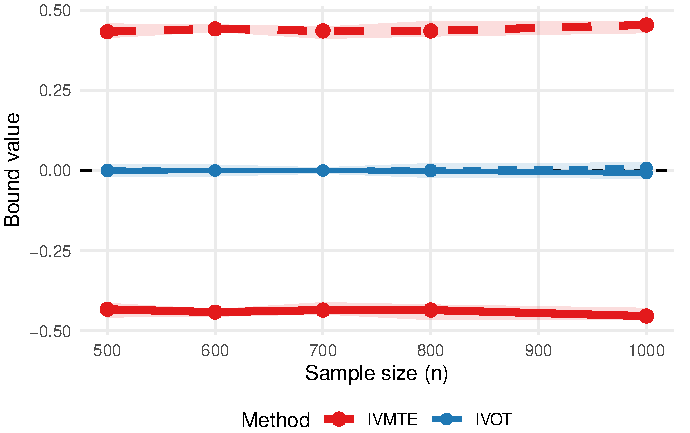
\includegraphics[width=0.75\linewidth]{figures/example3_1_bounds.pdf}
        \caption{Bounds of the moment relaxation approach and the CCOT approach by different sample sizes. Each data point is an average of 20 runs. In the experiment $M=1$, i.e., $y_{\max}=1, y_{\min}=-1$. }
        \label{fig:example3_1}
    \end{figure}
\end{example}

\section{Proofs of the Reduction Propositions}\label{oa:reductions}

This section proves the three closed-form rewritings on which the estimation procedures of \cref{sec:est_inf} are built. Each is an algebraic reduction of an expression already displayed in the main text, and none of the arguments below is used anywhere else.

\subsection{Proof of \cref{prop:discrete_reduction}}\label{app:closed_form_rewriting}

The nuisance components $\gamma_{\text{full},k}, \gamma_{j,k}, \gamma_K, J_{\text{full},k}, J_{j,k}, \Delta_K$ and the relative threshold $\kappa_{j,k}$ are defined in \cref{sec:est_inf} immediately preceding \cref{prop:discrete_reduction}; we refer to those formulas throughout this proof.

\begin{proof}[Proof of \cref{prop:discrete_reduction}]
    By \cref{thm:covariate_continuous_lower_bound} specialized to a finite instrument (every conditional LIV interval degenerate), it suffices to rewrite the conditional integral $\int_0^1 Q_{Y,k\mid X}(u)\,Q_{\omega,k\mid X}(1-u)\,\mathrm{d}u$ as an observable finite weighted sum. Fix $X$. On each baseline interval $(p_k(X), p_{k+1}(X))$ the weight function $\omega(X,u)$ is a non-increasing step function. On the sub-interval $(q_{j-1,k}(X),q_{j,k}(X))$, $j=1,\ldots,l_k$, exactly the current-bin instruments in $\bigcup_{l=j}^{l_k}T_{l,k}$ and all instruments whose alternative propensity lies in a strictly higher bin contribute to the first probability in $\omega$, whereas baseline propensities in strictly higher bins contribute to the second. Thus, up to the irrelevant boundary values,
    \begin{multline*}
        \omega(X,u) = \mathbb{P}_{\text{obs}}\!\left(Z \in \bigcup_{l=j}^{l_k} T_{l,k} \mathrel{\big|} X\right) + \mathbb{P}_{\text{obs}}\!\left(Z \in \bigcup_{i=k+1}^K \bigcup_{l=0}^{l_i} T_{l,i} \mathrel{\big|} X\right) \\
        - \mathbb{P}_{\text{obs}}\!\left(Z \in \bigcup_{i=k+1}^K S_i \mathrel{\big|} X\right),\quad u\in(q_{j-1,k},q_{j,k}).
    \end{multline*}
    Regrouping, the step-function value on the relevant slice is $\gamma_{\text{full},k}(X)+\gamma_{j,k}(X)$: the first term acts on the entire baseline interval and the second is the additional current-bin mass. Multiplying by $Q_{Y,k\mid X}$ and summing the nested current-bin contributions over the normalized sub-intervals yields
    \begin{multline*}
        (p_{k+1}(X) - p_k(X)) \int_0^1 Q_{Y,k\mid X}(u)\,Q_{\omega,k\mid X}(1-u)\,\mathrm{d}u \\
        = \gamma_{\text{full},k}(X)\, J_{\text{full},k}(X) + \sum_{j=1}^{l_k}\gamma_{j,k}(X)\, J_{j-1,k}(X),
    \end{multline*}
    where we used
    \begin{equation*}
        J_{\text{full},k}(X) = (p_{k+1}(X)-p_k(X))\,\mathbb{E}_{\mu_{1,k\mid X}}[Y] = (p_{k+1}(X)-p_k(X))\int_0^1 Q_{Y,k\mid X}(u)\,\mathrm{d}u
    \end{equation*}
    and the definition of $J_{j-1,k}$.

    The trivial-bound term on the tail $(p_K(X), 1]$ simplifies for the PRTE weight: since $\omega(X,u) = \mathbb{P}_{\text{obs}}(u < q(Z,X) \mid X) \geqslant 0$ for $u > p_K(X)$, we have $\int_{p_K(X)}^1 (y_{\min}\max\{0,\omega\} + y_{\max}\min\{0,\omega\})\,\mathrm{d}u = y_{\min}\int_{p_K(X)}^1 \omega(X,u)\,\mathrm{d}u$, which equals $\Delta_K(X)$ by Fubini. Taking the outer expectation over $X$ and summing over $k$ yields~(\ref{eq:target_discrete_iv}).

    The corresponding representation for the upper bound is obtained by the symmetric argument with $Q_{\omega,k\mid X}(1-t)$ replaced by $Q_{\omega,k\mid X}(t)$ in the OT term and $y_{\min}, y_{\max}$ swapped in the tail.
\end{proof}

\subsection{Proof of \cref{prop:J_specialization}}\label{app:J_specialization}

\begin{proof}[Proof of part (i).] Fix $k$ and $j \in \{0,\dots,l_k-1\}$. By the change of variables $u = F_{\mu_{1,k\mid X}}(y)$, continuity of $\mu_{1,k\mid X}$ at $\nu_{j,k}(X)$ and $\nu_{j+1,k}(X)$ gives $F_{\mu_{1,k\mid X}}(\nu_{j,k}(X)) = \kappa_{j,k}(X)$ and $F_{\mu_{1,k\mid X}}(\nu_{j+1,k}(X)) = \kappa_{j+1,k}(X)$ almost surely. Therefore,
\begin{align*}
    \int_{\kappa_{j,k}(X)}^{\kappa_{j+1,k}(X)} Q_{Y,k\mid X}(u)\,\mathrm{d}u &= \int_{\nu_{j,k}(X)}^{\nu_{j+1,k}(X)} y\, \mathrm{d}F_{\mu_{1,k\mid X}}(y) \\
    &= \mathbb{E}_{\mu_{1,k\mid X}}\!\big[Y\,\indicator\!\big(\nu_{j,k}(X) < Y \leqslant \nu_{j+1,k}(X)\big)\big],
\end{align*}
where the second equality uses the continuity of $\mu_{1,k\mid X}$ at the two boundary points to include/exclude boundary atoms without ambiguity. Multiplying by $p_{k+1}(X)-p_k(X)$ yields~(\ref{eq:J_cexpectation}).
\end{proof}

\begin{proof}[Proof of part (ii).] Suppose $Y \in \{0,1\}$. Let $\theta_k(X) \coloneqq \mathbb{E}_{\mu_{1,k\mid X}}[Y]$ denote the complier success probability on the $k$-th interval. By the definition of the identified complier measure \citep[cf.][]{angrist1995identification}, $(p_{k+1}(X)-p_k(X))\,\theta_k(X) = \mathbb{E}_{\text{obs}}[YW \mid Z \in S_{k+1}, X] - \mathbb{E}_{\text{obs}}[YW \mid Z \in S_k, X] = P_{1,k+1}(X) - P_{1,k}(X)$, so $J_{\text{full},k}(X) = P_{1,k+1}(X) - P_{1,k}(X)$.

Since $Y \in \{0,1\}$, the conditional quantile function is the step function $Q_{Y,k\mid X}(u) = \indicator(u \geqslant 1 - \theta_k(X))$. Equivalently, $Q_{Y,k\mid X}(u) = 1$ iff $u(p_{k+1}(X) - p_k(X)) + p_k(X) \geqslant p_{k+1}(X) - J_{\text{full},k}(X)$, i.e., the corresponding propensity value $v = p_k(X) + u(p_{k+1}(X)-p_k(X))$ lies in the interval $[p_{k+1}(X) - J_{\text{full},k}(X),\, p_{k+1}(X)]$. Writing $J_{j-1,k}(X)$ as a length in the original propensity scale, it equals the length of the intersection of $[q_{j-1,k}(X), q_{j,k}(X)]$ with $[p_{k+1}(X) - J_{\text{full},k}(X),\, p_{k+1}(X)]$:
\begin{equation*}
    J_{j-1,k}(X) = \max\!\Big(0,\; q_{j,k}(X) - \max\!\big(q_{j-1,k}(X),\; p_{k+1}(X) - J_{\text{full},k}(X)\big)\Big) = h_{j,k}^{-}(X).
\end{equation*}
Substituting into~(\ref{eq:target_discrete_iv}) yields~(\ref{eq:binary_lower_bound}).
\end{proof}

\subsection{Proof of \cref{prop:continuous_reduction}}\label{app:procedure_fubini}

\begin{proof}[Proof of \cref{prop:continuous_reduction}]
    Because $\mathcal{Z}$ is compact and connected and $z \mapsto p(z,X)$ is continuous by \cref{asp:continuity_p}, its image is a closed interval for almost every $X$, so \cref{thm:covariate_continuous_lower_bound} specializes with $K_X = 1$ and conditional LIV interval $[\underline{p}(X),\overline{p}(X)]$. We derive the three terms of~(\ref{eq:continuous_simplified_target}) in turn. Substituting the explicit form of the weight function,
    \begin{equation*}
        \omega(x,u) = \mathbb{E}_{Z \mid X}[\indicator (u \leqslant q(Z,X)) - \indicator (u \leqslant p(Z,X)) \mid X=x],
    \end{equation*}
    and applying Fubini's theorem to swap the order of integration, we handle each term separately.

    \textbf{First term (quantile integral on the gap $(0,\underline{p}(X))$).} For $\underline{p}(X)>0$, substitute the weight function, swap expectations, and use the change of variables $v=\underline{p}(X)u$. Because $P\ge \underline{p}(X)$ conditional on $X$, the baseline indicator equals one throughout this gap. Thus
    \begin{align*}
        \mathbb{E}_{X}&\!\left[ \underline{p}(X)\int_{0}^{1} Q_{1,\underline p\mid X}(u)\omega(X, \underline{p}(X)u)\, \mathrm{d}u \right] \\
        &= \mathbb{E}_{Z,X}\!\left[ \underline{p}(X)\int_{0}^{1} Q_{1,\underline p\mid X}(u)\big(\indicator (\underline{p}(X)u \leqslant q(Z,X)) - 1\big)\, \mathrm{d}u \right] \\
        &= -\mathbb{E}_{Z,X}\!\left[ \int_{\min\{\underline{p}(X),\,q(Z,X)\}}^{\underline{p}(X)} Q_{1,\underline p\mid X}\!\left({v}/{\underline{p}(X)}\right)\, \mathrm{d}v \right].
    \end{align*}
    Both sides are zero when $\underline{p}(X)=0$, which justifies the convention in the proposition.

    \textbf{Second term ($g_1$ difference on the LIV interval).} The structural integral representation gives $g_1(u,x)=\int_0^u\mathbb E[Y(1)\mid U=s,X=x]\,\mathrm ds$, so $g_1(\cdot,x)$ is absolutely continuous. Hence, for any $r\in[0,1]$,
    \[
        \int_{\underline{p}(X)}^{\overline{p}(X)} \partial_u g_1(u,X)\indicator(u\le r)\,\mathrm du
        =g_1\!\left(\min\{\overline{p}(X),\max\{\underline{p}(X),r\}\},X\right)-g_1(\underline{p}(X),X).
    \]
    Applying this identity first with $r=q(Z,X)$ and then with $r=P$ is essential when $q(Z,X)<\underline{p}(X)$. Since $P\in[\underline{p}(X),\overline{p}(X)]$, the two lower-endpoint terms cancel and give
    \begin{align*}
       \mathbb{E}_{X}\!\left[ \int_{\underline{p}(X)}^{\overline{p}(X)} \frac{\partial g_1(u, X)}{\partial u} \omega(X,u)\, \mathrm{d}u \right]
        &= \mathbb{E}_{Z,X}\!\left[g_1\big(q^{\mathrm{tr}}(Z,X),X\big)-g_1\big(P,X\big)\right].
    \end{align*}

    \textbf{Third term (trivial bound on $(\overline{p}(X),1]$).} Since $P\le \overline{p}(X)$, the baseline indicator vanishes on this tail and $\omega(X,u)=\mathbb P(u\le q(Z,X)\mid X)\ge0$. Therefore
    \begin{align*}
        y_{\min} \mathbb{E}_{X}\!\left[\int_{\overline{p}(X)}^{1} \omega(X,u)\, \mathrm{d}u\right]
        =y_{\min}\mathbb E_{Z,X}\!\left[(q(Z,X)-\overline{p}(X))_+\right].
    \end{align*}
    Aggregating the three components yields~(\ref{eq:continuous_simplified_target}). The upper-bound representation replaces the countermonotonic boundary coupling by the comonotonic coupling and swaps $y_{\min}$ for $y_{\max}$ in the trivial tail.
\end{proof}

\section{Moment Condition and Neyman Orthogonality of the Discrete-Instrument Scores}\label{oa:orthogonality}

This section proves \cref{lem:orthogonality_discrete}. Both parts are term-by-term calculations that repeatedly apply the tower property to inverse-probability-weighted residuals with zero conditional mean.

Throughout, $\eta_0$ denotes the vector of true nuisance parameter values and $\theta_0 = \underline{\theta}_{\omega,1}$ the true parameter value. For a functional $\Phi(\eta)$ and a perturbation direction $\delta$ in the same function space as $\eta$, we write $\partial_\delta \Phi(\eta) \coloneqq \frac{\mathrm{d}}{\mathrm{d}t}\Phi(\eta + t\,\delta)\big|_{t=0}$ for the Gateaux (directional) derivative; when the perturbation is along a single nuisance component $\eta_\alpha$, we write $\partial_{\eta_\alpha}$ for brevity.

\subsection{Continuous Outcome}\label{oa:orthogonality_continuous}

Recall the target functional:
\begin{equation}\label{eq:pf_target_recall}
    \theta_0 = \mathbb{E}\Bigg[\sum_{k=0}^{K-1}\bigg(\gamma_{\mathrm{full},k}(X)\,J_{\mathrm{full},k}(X) + \sum_{j=1}^{l_k} \gamma_{j,k}(X)\,J_{j-1,k}(X)\bigg) + \Delta_K(X)\Bigg],
\end{equation}
and the total Neyman-orthogonal score assembled from the components of \cref{app:scores_continuous}:
\begin{equation}\label{eq:pf_total_score}
    \psi(O;\eta) = \sum_{k=0}^{K-1}\Bigl(\psi_{\mathrm{full},k}^{\mathrm{prod}}(O;\eta) + \sum_{j=1}^{l_k}\psi_{j,k}^{\mathrm{prod}}(O;\eta)\Bigr) + \psi_{\Delta_K}(O;\eta),
\end{equation}
where each product score debiases the corresponding term in the target. Specifically, $\psi_{j,k}^J(O;\eta)$ is the uncentered orthogonal score for the conditional integral component $\mathbb{E}[J_{j,k}(X)]$, and the product score for $\mathbb{E}[\gamma_{j,k}(X)\,J_{j-1,k}(X)]$ is:
\begin{equation}\label{eq:pf_prod_score_recall}
    \psi_{j,k}^{\mathrm{prod}}(O;\eta) = \gamma_{j,k}(X)\,\psi_{j-1,k}^J(O;\eta) + J_{j-1,k}(X)\Bigl(\indicator\bigl(Z \in {\textstyle\bigcup_{l=j}^{l_k}} T_{l,k}\bigr) - \gamma_{j,k}(X)\Bigr),
\end{equation}
and symmetrically for $\psi_{\mathrm{full},k}^{\mathrm{prod}}(O;\eta)$.

\begin{proof}[Proof of \cref{lem:orthogonality_discrete}\textup{(i)}]
\medskip
\noindent\textbf{Moment condition.}
We show $\mathbb{E}[\psi(O;\eta_0)] = \theta_0$. All influence function correction terms in the score are inverse-probability-weighted residuals of the general form
\[
    \frac{\indicator(Z \in S_k)}{\pi_k(X)}\,W\bigl(g(Y,X) - \mathbb{E}[g(Y,X) \mid X, Z \in S_k, W\!=\!1]\bigr).
\]
By the tower property, conditioning first on $(X,Z)$: when $Z \in S_k$, we have $p(Z,X) = p_k(X)$, so $\mathbb{E}[W \mid X, Z \in S_k] = p_k(X)$. It follows that
\[
    \mathbb{E}\Big[\frac{\indicator(Z \in S_k)}{\pi_k(X)}\,W\bigl(g - \mathbb{E}[g \mid X, S_k, W\!=\!1]\bigr)\Big] = \mathbb{E}\Big[\frac{\indicator(Z \in S_k)}{\pi_k(X)}\,p_k(X)\cdot 0\Big] = 0.
\]
Applying this identity to each correction term, $\mathbb{E}[IF_{J^\pm}(O)] = 0$ and $\mathbb{E}[IF_{M_{j,k}^\pm}(O)] = 0$ at $\eta_0$. The quantile correction term in $\psi_{j,k}^J$ contains the factor $p_{k+1}(X)M_{j,k}^+(X) - p_k(X)M_{j,k}^-(X) - (q_{j,k}(X) - p_k(X))$, which vanishes at $\eta_0$ by the conditional moment equation
\begin{equation}\label{eq:pf_quantile_moment_dml}
    \begin{split}
        &p_{k+1}(X)\,\mathbb{E}[\indicator(Y \leqslant \nu_{j,k}(X)) \mid X, S_{k+1}, W\!=\!1]\\
        & \quad\quad \quad \quad - p_k(X)\,\mathbb{E}[\indicator(Y \leqslant \nu_{j,k}(X)) \mid X, S_k, W\!=\!1] - (q_{j,k}(X) - p_k(X)) = 0
    \end{split}
\end{equation}
which defines $\nu_{j,k}$ for $j\geqslant1$; the boundary value $\nu_{0,k}=y_{\min}$ is fixed. The propensity score correction terms $\frac{\indicator(Z \in S_k)}{\pi_k(X)}(W - p_k(X))$ and the pooled policy-level residuals $R_{q,j,k}$ likewise have zero mean by the same tower-property argument. Consequently,
\begin{align*}
    \mathbb{E}[\psi_{j,k}^J(O;\eta_0)] &= \mathbb{E}[J_{j,k}(X)], & \mathbb{E}[\psi_{\mathrm{full},k}^J(O;\eta_0)] &= \mathbb{E}[J_{\mathrm{full},k}(X)].
\end{align*}
For the product scores, substituting~(\ref{eq:pf_prod_score_recall}) and using $\mathbb{E}[\indicator(Z \in \bigcup_{l=j}^{l_k} T_{l,k}) - \gamma_{j,k}(X)] = 0$:
\begin{align*}
    \mathbb{E}[\psi_{j,k}^{\mathrm{prod}}(O;\eta_0)] &= \mathbb{E}\bigl[\gamma_{j,k}(X)\,\underbrace{\mathbb{E}[\psi_{j-1,k}^J(O;\eta_0) \mid X]}_{= J_{j-1,k}(X)}\bigr] + \mathbb{E}\bigl[J_{j-1,k}(X)\,\underbrace{\mathbb{E}[\indicator(\cdots) - \gamma_{j,k}(X) \mid X]}_{= 0}\bigr] \\
    &= \mathbb{E}[\gamma_{j,k}(X)\,J_{j-1,k}(X)],
\end{align*}
and symmetrically $\mathbb{E}[\psi_{\mathrm{full},k}^{\mathrm{prod}}(O;\eta_0)] = \mathbb{E}[\gamma_{\mathrm{full},k}(X)\,J_{\mathrm{full},k}(X)]$. The same reasoning yields $\mathbb{E}[\psi_{\Delta_K}(O;\eta_0)] = \mathbb{E}[\Delta_K(X)]$. Summing over all components and comparing with~(\ref{eq:pf_target_recall}) gives $\mathbb{E}[\psi(O;\eta_0)] = \theta_0$.

\medskip
\noindent\textbf{Neyman orthogonality of $\psi_{j,k}^J$.}
We show that the Gateaux derivative $\partial_t\,\mathbb{E}[\psi_{j,k}^J(O;\eta_0 + t\,\delta)]|_{t=0}$ vanishes for all perturbation directions~$\delta$. We group the nuisance parameters by type and check orthogonality with respect to each group.

\textbf{Conditional expectations $(J_{j,k}^\pm, M_{j,k}^\pm)$.}
Consider a perturbation $J_{j,k}^+(X) \to J_{j,k}^+(X) + t\,\delta J^+(X)$. The plug-in term $J_{j,k} = p_{k+1}\,J_{j,k}^+ - p_k\,J_{j,k}^-$ contributes $+\mathbb{E}[p_{k+1}(X)\,\delta J^+(X)]$, while the IPW correction $IF_{J^+}$ contributes $-\mathbb{E}\bigl[\frac{\indicator(Z \in S_{k+1})}{\pi_{k+1}(X)}\,p_{k+1}(X)\,\delta J^+(X)\bigr]$. These cancel because
\[
    \mathbb{E}\!\left[\frac{\indicator(Z \in S_{k+1})}{\pi_{k+1}(X)} \mathrel{\bigg|} X\right] = \frac{\mathbb{P}(Z \in S_{k+1} \mid X)}{\pi_{k+1}(X)} = 1.
\]
For $J_{j,k}^-$ the plug-in derivative is $-p_k\delta J^-$, while differentiating $-IF_{J^-}$ gives $+p_k\delta J^-$. For $M_{j,k}^+$, the plug-in part of the quantile moment gives $\nu_{j,k}p_{k+1}\delta M^+$ and differentiating $\nu_{j,k}IF_{M_{j,k}^+}$ gives its negative; the minus-side and $j+1$ terms cancel in the same way, with their displayed signs. Thus every conditional-expectation direction cancels explicitly.

\textbf{Instrument assignment probabilities $(\pi_k, \pi_{k+1})$.}
Perturbing $\pi_{k+1}(X) \to \pi_{k+1}(X) + t\,\delta\pi(X)$ introduces a factor $-\delta\pi(X)/\pi_{k+1}(X)^2$ in the IPW terms. For any such IPW term $\indicator(Z \in S_{k+1})\,\pi_{k+1}(X)^{-1}\,W\,(g(O) - \bar{g}(X))$, the first-order contribution is
\[
    -\mathbb{E}\!\left[\frac{\indicator(Z \in S_{k+1})}{\pi_{k+1}(X)^2}\,\delta\pi(X)\,W\,(g(O) - \bar{g}(X))\right].
\]
Conditioning on $(X,Z)$ with $Z \in S_{k+1}$, we have $\mathbb{E}[W(g(O) - \bar{g}(X)) \mid X, Z \in S_{k+1}] = p_{k+1}(X) \cdot 0 = 0$ at $\eta_0$, so the Gateaux derivative vanishes. The argument for $\delta\pi_k$ is identical when $k\geqslant1$; there is no $\pi_0$ direction.

\textbf{Propensity scores $(p_k, p_{k+1})$.}
For $k\geqslant1$, a perturbation $p_k(X) \to p_k(X) + t\,\delta p_k(X)$ generates first-order contributions from three sources (all multiplied by $\delta p_k(X)$ inside $\mathbb{E}[\cdot]$). There is no such direction at $k=0$ because $p_0\equiv0$ is fixed:
\begin{enumerate}
    \item[(i)] The plug-in term $J_{j,k} = p_{k+1}\,J_{j,k}^+ - p_k\,J_{j,k}^-$, contributing $-J_{j,k}^-(X)$;
    \item[(ii)] The quantile correction terms $\nu_{j,k}(\cdots) - \nu_{j+1,k}(\cdots)$, contributing $\nu_{j,k}(X)(\indicator(j\geqslant1) - M_{j,k}^-(X)) - \nu_{j+1,k}(X)(1 - M_{j+1,k}^-(X))$. At $j=0$, the first constant is absent because $q_{0,k}-p_k\equiv0$;
    \item[(iii)] The Riesz representer correction $\alpha_{p_k}(X)\frac{\indicator(Z \in S_k)}{\pi_k(X)}(W - p_k(X))$, contributing $-\alpha_{p_k}(X)$.
\end{enumerate}
Substituting the definition
\[
    \alpha_{p_k} = -J_{j,k}^- - \nu_{j,k}\,M_{j,k}^- + \nu_{j+1,k}\,M_{j+1,k}^- + \indicator(j\geqslant1)\nu_{j,k} - \nu_{j+1,k}
\]
and collecting terms:
\begin{align*}
    &\bigl(-J_{j,k}^-\bigr) + \bigl(\indicator(j\geqslant1)\nu_{j,k} - \nu_{j,k}\,M_{j,k}^- - \nu_{j+1,k} + \nu_{j+1,k}\,M_{j+1,k}^-\bigr) \\
    &\quad - \bigl(-J_{j,k}^- - \nu_{j,k}\,M_{j,k}^- + \nu_{j+1,k}\,M_{j+1,k}^- + \indicator(j\geqslant1)\nu_{j,k} - \nu_{j+1,k}\bigr) = 0.
\end{align*}
The calculation for $\delta p_{k+1}$, using $\alpha_{p_{k+1}} = J_{j,k}^+ + \nu_{j,k}\,M_{j,k}^+ - \nu_{j+1,k}\,M_{j+1,k}^+$, is identical.

\textbf{Quantile thresholds $(\nu_{j,k}, \nu_{j+1,k})$.}
A perturbation is considered only for estimated thresholds. In particular, $\nu_{0,k}=y_{\min}$ is fixed and has no nuisance direction.
A perturbation $\nu_{j,k}(X) \to \nu_{j,k}(X) + t\,\delta\nu(X)$ affects the score through two channels.

\textbf{Channel~(a): indicator boundaries.} The indicator $\indicator(\nu_{j,k}(X) \leqslant Y)$ appears inside $IF_{J^\pm}$ and $IF_{M_{j,k}^\pm}$. For a generic relevant conditional law $F$ and $a_t=\nu+t\,\delta\nu$, the combined boundary change from the truncated first-moment correction and its quantile-moment correction is, up to its orientation,
\[
    \int_{\nu}^{a_t}(a_t-y)\,\mathrm{d}F(y).
\]
If the density of $F$ is bounded by $C$ in the stated neighborhood, then
\[
    \left|\int_{\nu}^{a_t}(a_t-y)\,\mathrm{d}F(y)\right|
    \leqslant C|a_t-\nu|^2.
\]
The oriented-integral convention covers $a_t<\nu$. Applying this bound to the plus and minus conditional laws shows that the combined boundary contribution is $O(t^2\delta\nu^2)$ and therefore has derivative zero at $t=0$.

\textbf{Channel~(b): explicit multiplicative factor.} The term $\nu_{j,k}(X)\bigl(p_{k+1} M_{j,k}^+ - p_k M_{j,k}^- - (q_{j,k} - p_k)\bigr)$ contributes $\delta\nu(X)$ times the conditional moment equation~(\ref{eq:pf_quantile_moment_dml}), which vanishes at $\eta_0$. The dependence of $\alpha_{p_k}$ and $\alpha_{p_{k+1}}$ on $\nu_{j,k}$ is absorbed by the zero-mean residuals: for any $L_2$ function $h(X)$,
\[
    \mathbb{E}\!\left[h(X)\,\frac{\indicator(Z \in S_k)}{\pi_k(X)}\bigl(W - p_k(X)\bigr)\right] = \mathbb{E}\!\left[h(X)\,\frac{\pi_k(X)}{\pi_k(X)}\cdot 0\right] = 0.
\]
The local density bound gives the quadratic control above. The treatment of $\delta\nu_{j+1,k}$ is symmetric.

\textbf{Alternative policy propensity $(q_{j,k})$.}
For $j\geqslant1$, use the pooled representation $q_{j,k}(X)=\mathbb E[q(Z,X)\mid Z\in T_{j,k},X]$. At the population law, all the instrument-specific policy propensities in $T_{j,k}$ equal this common value. Consequently, perturbations of the conditional instrument probabilities have no first-order effect on the pooled value, while perturbing the propensity functions induces
\[
    \delta q_{j,k}(X)
    =\frac{1}{\tau_{j,k}(X)}
      \sum_{z\in T_{j,k}}\pi(z,X)
      \frac{\partial\phi}{\partial p}(z,X,p(z,X))\,\delta p(z,X).
\]
At $j=0$, $T_{0,k}=\emptyset$ and the boundary $q_{0,k}=p_k$ is handled by the corrected $p_k$ representer above. For $j\geqslant1$, the first-order contributions are:
\begin{align*}
    \text{from quantile correction}&: \quad -\mathbb{E}\bigl[\nu_{j,k}(X)\,\delta q_{j,k}(X)\bigr], \\
    \text{from differentiating the policy residual}&: \quad +\mathbb{E}\bigl[\nu_{j,k}(X)\,\delta q_{j,k}(X)\bigr].
\end{align*}
The pooled correction itself has mean zero at the truth. Differentiating its residuals gives
\[
    \partial_t\mathbb E[-\nu_{j,k}(X)R_{q,j,k}(O)]\big|_{t=0}
    =\mathbb E[\nu_{j,k}(X)\,\delta q_{j,k}(X)],
\]
because $\mathbb E[\indicator(Z=z)\mid X]=\pi(z,X)$. Derivatives of the coefficients multiply zero-mean residuals and therefore vanish. The two displayed contributions cancel, and the treatment of $q_{j+1,k}$ is symmetric.

The simplex restriction is essential for the preceding pooled representation. Along a within-set share perturbation $a_{j,k}(z,X)\mapsto a_{j,k}(z,X)+t\,\delta a_z(X)$, admissible directions satisfy $\sum_{z\in T_{j,k}}\delta a_z(X)=0$. Since $q(z,X)=q_{j,k}(X)$ for every $z\in T_{j,k}$ at the population law,
\[
    \partial_t\sum_{z\in T_{j,k}}(a_{j,k}(z,X)+t\,\delta a_z(X))q(z,X)\Big|_{t=0}
    =q_{j,k}(X)\sum_{z\in T_{j,k}}\delta a_z(X)=0.
\]
With estimated instrument-specific policy values, the remaining share term is $\sum_z(\hat a_z-a_z)(\hat q(z,X)-q_{j,k}(X))$, a product of two nuisance errors. A perturbation of $\tau_{j,k}$ affects only the factor $1/\tau_{j,k}$ in $R_{q,j,k}$; its derivative multiplies the conditionally mean-zero numerator $\sum_{z\in T_{j,k}}\phi_p(z,X,p(z,X))\indicator(Z=z)(W-p(z,X))$ and is therefore zero at the truth.

This establishes orthogonality for $\psi_{j,k}^J$.

\medskip
\noindent\textbf{Neyman orthogonality of the remaining components.}
For $\psi_{\mathrm{full},k}^J$, a perturbation of $J_{\mathrm{full},k}^+$ contributes $p_{k+1}\delta J^+$ through the plug-in and $-p_{k+1}\delta J^+$ through its outcome residual. A perturbation of $p_{k+1}$ contributes $J_{\mathrm{full},k}^+\delta p_{k+1}$ through the plug-in and its negative through the propensity residual. The minus-side terms cancel identically when $k\geqslant1$, and denominator perturbations in $\pi_k,\pi_{k+1}$ multiply conditionally mean-zero residuals. Hence $\psi_{\mathrm{full},k}^J$ is orthogonal in every nuisance direction.

For the product scores, we invoke the chain rule for influence functions. The preceding cancellations hold conditionally on $X$: at $\eta_0$, $\mathbb E[\psi_{j-1,k}^J(O;\eta_0)\mid X]=J_{j-1,k}(X)$, and the Gateaux derivative of this conditional moment is zero in every nuisance direction already considered. Moreover, $\indicator(Z \in \bigcup_{l=j}^{l_k} T_{l,k}) - \gamma_{j,k}(X)$ is the conditional influence function for $\gamma_{j,k}(X) = \mathbb{P}(Z \in \bigcup_{l=j}^{l_k} T_{l,k} \mid X)$. Therefore, the product score~(\ref{eq:pf_prod_score_recall})
\[
    \psi_{j,k}^{\mathrm{prod}} = \gamma_{j,k}(X)\,\psi_{j-1,k}^J(O;\eta) + J_{j-1,k}(X)\bigl(\indicator(Z \in {\textstyle\bigcup_{l=j}^{l_k}} T_{l,k}) - \gamma_{j,k}(X)\bigr)
\]
is orthogonal for the product functional $\mathbb{E}[\gamma_{j,k}(X)\,J_{j-1,k}(X)]$. We treat the two groups of nuisance directions separately. First, let $\eta_\alpha$ be any component other than $\gamma_{j,k}$. Then $\gamma_{j,k}$ and the indicator residual do not vary, so
\begin{multline*}
    \partial_{\eta_\alpha}\mathbb{E}[\psi_{j,k}^{\mathrm{prod}}] = \mathbb{E}\bigl[\gamma_{j,k}(X)\,\underbrace{\partial_{\eta_\alpha}\mathbb{E}[\psi_{j-1,k}^J \mid X]}_{=\,0}\bigr] \\
    + \mathbb{E}\bigl[\partial_{\eta_\alpha}J_{j-1,k}(X)\,\underbrace{\mathbb{E}[\indicator(\cdots) - \gamma_{j,k}(X) \mid X]}_{=\,0}\bigr] = 0,
\end{multline*}
where the first expectation vanishes by the conditional orthogonality just established. Second, for the direction $\gamma_{j,k} \mapsto \gamma_{j,k} + t\,\delta\gamma$, the derivative contributions of the explicit prefactor and the residual cancel:
\[
    \partial_t\,\mathbb{E}\bigl[(\gamma_{j,k}+t\,\delta\gamma)\psi_{j-1,k}^J + J_{j-1,k}(\indicator(\cdots) - \gamma_{j,k} - t\,\delta\gamma)\bigr]\Big|_{t=0}
    = \mathbb{E}[\delta\gamma\,J_{j-1,k}] - \mathbb{E}[\delta\gamma\,J_{j-1,k}] = 0,
\]
using $\mathbb{E}[\psi_{j-1,k}^J \mid X] = J_{j-1,k}(X)$ at $\eta_0$. For the full-interval product, the residual is
\[
\indicator\!\left(Z\in\bigcup_{m=k+1}^K\bigcup_{l=0}^{l_m}T_{l,m}\right)
-\indicator\!\left(Z\in\bigcup_{m=k+1}^KS_m\right)-\gamma_{\mathrm{full},k}(X),
\]
whose conditional mean is zero by the definition of $\gamma_{\mathrm{full},k}$. Therefore its coefficient and residual derivatives cancel exactly as in~(\ref{eq:pf_prod_score_recall}), even though $\gamma_{\mathrm{full},k}$ is signed.

For $\psi_{\Delta_K}$, write
\begin{equation*}
    A_K=\Bigl\{Z\in\bigcup\nolimits_{j=1}^{l_K}T_{j,K}\Bigr\}.
\end{equation*}
A perturbation of $p_K$ contributes $-y_{\min}\mathbb E[\gamma_K(X)\,\delta p_K(X)]$ through the plug-in term and the opposite quantity through differentiation of the $p_K$ residual. For an instrument-specific direction $p(z,X)\mapsto p(z,X)+t\,\delta p(z,X)$, the plug-in derivative is
\[
y_{\min}\mathbb E\!\left[\indicator(A_K)\phi_p(Z,X,p(Z,X))\delta p(Z,X)\right],
\]
and differentiation of the policy residual gives its negative. Perturbations of $\pi_K$ and of the coefficient $\gamma_K$ multiply the conditionally mean-zero $p_K$ residual, while derivatives of $\phi_p$ multiply $W-p(Z,X)$ and also have conditional mean zero. Thus every first-order direction in $\psi_{\Delta_K}$ cancels.

\end{proof}

\subsection{Binary Outcome}\label{oa:orthogonality_binary}

\begin{proof}[Proof of \cref{lem:orthogonality_discrete}\textup{(ii)}]
Recall the target functional~(\ref{eq:binary_lower_bound}) and the orthogonal score~(\ref{eq:binary_score}), which decomposes as $\psi = \sum_{k}(\psi_{\mathrm{full},k}^{\mathrm{prod}} + \sum_{j}\psi_{j,k}^{\mathrm{prod}}) + \psi_{\Delta_K}$.
\medskip
\noindent\textbf{Moment condition.}
We show $\mathbb{E}[\psi(O;\eta_0)] = \theta_0$. The residuals $R_{P,k}$ and $R_{p,k}$ have conditional mean zero because $P_{1,k}(X)=\mathbb E[YW\mid Z\in S_k,X]$ and $p_k(X)=\mathbb E[W\mid Z\in S_k,X]$. The pooled policy residual also satisfies
\begin{multline*}
\mathbb E[R_{q,j,k}(O)\mid X] \\
=\frac1{\tau_{j,k}(X)}\sum_{z\in T_{j,k}}\phi_p(z,X,p(z,X))\,\mathbb P(Z=z\mid X)\,\mathbb E[W-p(z,X)\mid Z=z,X]
=0.
\end{multline*}
Thus every correction in $\psi_{j,k}^h$ and $\psi_{\mathrm{full},k}^J$ has conditional mean zero, so $\mathbb{E}[\psi_{j,k}^h(O;\eta_0)\mid X] = h_{j,k}^-(X)$ and $\mathbb{E}[\psi_{\mathrm{full},k}^J(O;\eta_0)\mid X] = J_{\mathrm{full},k}(X)$. Writing $A_{j,k}=\{Z\in\bigcup_{l=j}^{l_k}T_{l,k}\}$, another application of the tower property gives
\begin{align*}
    \mathbb E[\psi_{j,k}^{\mathrm{prod}}(O;\eta_0)]
    &=\mathbb E\!\left[\gamma_{j,k}(X)\,\mathbb E[\psi_{j,k}^h(O;\eta_0)\mid X]
      +h_{j,k}^-(X)\,\mathbb E[\indicator(A_{j,k})-\gamma_{j,k}(X)\mid X]\right] \\
    &=\mathbb E[\gamma_{j,k}(X)h_{j,k}^-(X)].
\end{align*}
The same conditional calculation applies to the full-interval product score. Summing all components therefore gives $\mathbb{E}[\psi(O;\eta_0)] = \mathbb{E}[m(X;\eta_0)] = \theta_0$.

\medskip
\noindent\textbf{Neyman orthogonality.}
We must show $\partial_{\eta_\alpha}\mathbb{E}[\psi(O;\eta)]\big|_{\eta=\eta_0} = 0$ for each nuisance component $\eta_\alpha$. By the product score structure, it suffices to establish orthogonality of the component scores $\psi_{j,k}^h$ and $\psi_{\mathrm{full},k}^J$ with respect to $(P_{1,m},p_m,p(z,X),\pi_m,\tau_{j,k},a_{j,k})$, and then show that the product scores inherit orthogonality with respect to the $\gamma$ terms.

\textbf{Orthogonality of $\psi_{j,k}^h$ with respect to $P_{1,m}$.}
Consider a perturbation $P_{1,m} \to P_{1,m} + t\,\delta P_{1,m}(X)$. Since $h_{j,k}^-$ depends on $P_{1,m}$ only through $J_{\mathrm{full},k} = P_{1,k+1} - P_{1,k}$, the pathwise derivative is
\[
    \partial_t \mathbb{E}[h_{j,k}^-] \big|_{t=0} = \mathbb{E}\!\left[\alpha_{P,m}^{(j,k)}(X)\,\delta P_{1,m}(X)\right],
\]
where $\alpha_{P,k+1}^{(j,k)} = D_{j,k}^-$, $\alpha_{P,k}^{(j,k)} = -D_{j,k}^-$, and $\alpha_{P,m}^{(j,k)} = 0$ for $m \notin \{k,k{+}1\}$. Under \cref{asp:discrete_outcome_gap}, $D_{j,k}^- = \indicator(q_{j-1,k} < p_{k+1} - J_{\mathrm{full},k} < q_{j,k})$ is well-defined. The IPW correction $D_{j,k}^-(R_{P,k+1} - R_{P,k})$ in $\psi_{j,k}^h$ contributes
\begin{multline*}
    \partial_t \mathbb{E}\!\left[D_{j,k}^-\!\left(\frac{\indicator(Z \in S_{k+1})}{\pi_{k+1}}\bigl(YW - P_{1,k+1}\bigr) - \frac{\indicator(Z \in S_k)}{\pi_k}\bigl(YW - P_{1,k}\bigr)\right)\right]\bigg|_{t=0} \\
    = -\mathbb{E}\!\left[\alpha_{P,m}^{(j,k)}\,\delta P_{1,m}\right],
\end{multline*}
using $\mathbb{E}[\frac{\indicator(Z \in S_m)}{\pi_m} \mid X] = 1$, so the two contributions cancel. The same argument gives $\partial_{P_{1,m}}\mathbb{E}[\psi_{\mathrm{full},k}^J] = 0$ (with $\alpha_{P,k+1}^{(\mathrm{full},k)} = 1$ and $\alpha_{P,k}^{(\mathrm{full},k)} = -1$).

\noindent\textit{Remark (notation).} For $k\in\{0,\ldots,K-1\}$ and $j\in\{1,\ldots,l_k\}$, $\alpha_{P,k}^{(j,k)}(x)=-D_{j,k}^{-}(x)$ is the coefficient of the $P_{1,k}$ perturbation in the derivative of $h_{j,k}^{-}$, with the other nuisance arguments held fixed.


\textbf{Orthogonality of $\psi_{j,k}^h$ with respect to $p_m$ and $p(z,X)$.}
The propensity scores enter $h_{j,k}^-$ through three channels:

\begin{enumerate}[label=(\alph*)]
    \item the integration boundary $p_{k+1} - J_{\mathrm{full},k}$, corrected by $\alpha_{p,k+1}^{(j,k)} R_{p,k+1}$;
    \item the lower level-set boundary $q_{0,k} = p_k$ when $j = 1$, corrected by $\alpha_{p,k}^{(1,k)} R_{p,k}$;
    \item the alternative policy values $q_{j,k}$ and $q_{j-1,k}$ through the mapping $\phi(z,X,p(z,X))$, corrected by the policy terms involving $T_{j,k}$ and $T_{j-1,k}$.
\end{enumerate}

For channel (a), a perturbation $p_{k+1} \to p_{k+1} + t\,\delta p_{k+1}(X)$ shifts the boundary by $\delta p_{k+1}$, giving $\partial_t h_{j,k}^- = -D_{j,k}^-\,\delta p_{k+1}$. The correction $\alpha_{p,k+1}^{(j,k)} R_{p,k+1} = -D_{j,k}^- \cdot \frac{\indicator(Z \in S_{k+1})}{\pi_{k+1}}(W - p_{k+1})$ contributes $\partial_t \mathbb{E}[\alpha_{p,k+1}^{(j,k)} R_{p,k+1}] = D_{j,k}^-\,\delta p_{k+1}$, canceling the plug-in derivative.

For channel (b), when $j = 1$ and $E_{1,k}^- = 1$ (i.e., $p_k > p_{k+1} - J_{\mathrm{full},k}$), a perturbation of $p_k$ shifts $q_{0,k} = p_k$, giving $\partial_t h_{1,k}^- = -E_{1,k}^- I_{1,k}^-\,\delta p_k$. The correction $\alpha_{p,k}^{(1,k)} R_{p,k}$ contributes the matching cancellation.

For channel (c), the pooled derivative displayed in the continuous-outcome proof gives $\partial_t h_{j,k}^-=I_{j,k}^-\,\delta q_{j,k}$ for the upper boundary. The derivative of $I_{j,k}^-R_{q,j,k}$ is $-I_{j,k}^-\,\delta q_{j,k}$ and therefore cancels it. Symmetrically, when $E_{j,k}^-=1$, the correction through $R_{q,j-1,k}$ cancels the derivative through the lower boundary $q_{j-1,k}$.

\textbf{Denominators and within-set shares.}
A perturbation of $\pi_m$ differentiates only denominators in $R_{P,m}$ and $R_{p,m}$; each resulting term is a function of $X$ times a conditionally mean-zero residual, so its expectation is zero. The same argument applies to a perturbation of $\tau_{j,k}$ in $R_{q,j,k}$. Finally, admissible share directions satisfy $\sum_{z\in T_{j,k}}\delta a_z(X)=0$. At the truth, all $q(z,X)$ in $T_{j,k}$ equal $q_{j,k}(X)$, and hence
\[
\partial_t\sum_{z\in T_{j,k}}(a_{j,k}(z,X)+t\delta a_z(X))q(z,X)\Big|_{t=0}
=q_{j,k}(X)\sum_{z\in T_{j,k}}\delta a_z(X)=0.
\]
Thus the simplex-share direction has no first-order effect; with estimated $q(z,X)$ it contributes only the product $\sum_z(\hat a_z-a_z)(\hat q_z-q_{j,k})$.

\textbf{Inheritance by product scores.}
Recall that
\begin{equation*}
    \psi_{j,k}^{\mathrm{prod}} = \gamma_{j,k}\,\psi_{j,k}^h + h_{j,k}^-(\indicator(\cdots) - \gamma_{j,k}),
    \qquad \mathbb{E}[\indicator(\cdots) - \gamma_{j,k} \mid X] = 0 \ \text{ at } \eta_0,
\end{equation*}
while the preceding component-score cancellations hold conditionally on $X$. Hence any perturbation of a component-score nuisance
$(P_{1,m},\,p_m,\,p(z,X),\,\pi_m,\,\tau_{j,k},\,a_{j,k})$
yields
\[
    \partial_\eta \mathbb{E}[\psi_{j,k}^{\mathrm{prod}}]
    =\mathbb E\!\left[\gamma_{j,k}(X)\,\underbrace{\partial_\eta \mathbb{E}[\psi_{j,k}^h\mid X]}_{=\,0}
    +\partial_\eta h_{j,k}^-(X)\,\underbrace{\mathbb{E}[\indicator(\cdots) - \gamma_{j,k}(X) \mid X]}_{=\,0}\right]=0.
\]
For $\psi_{\mathrm{full},k}^{\mathrm{prod}}$, the same calculation uses the signed residual
\[
\indicator\!\left(Z\in\bigcup_{m=k+1}^K\bigcup_{l=0}^{l_m}T_{l,m}\right)
-\indicator\!\left(Z\in\bigcup_{m=k+1}^KS_m\right)-\gamma_{\mathrm{full},k}(X),
\]
whose conditional mean is zero. For $\psi_{\Delta_K}$, the $p_K$ plug-in derivative cancels the derivative of its $R_{p,K}$ correction, while each instrument-specific derivative through $q(z,X)=\phi(z,X,p(z,X))$ cancels the corresponding policy residual. Perturbations of $\pi_K$, $\gamma_K$, and the policy-derivative coefficient multiply conditionally mean-zero residuals. Hence $\psi_{\Delta_K}$ is also orthogonal in every nuisance direction.

\textbf{Perturbation of $\gamma_{j,k}$ and $\gamma_{\mathrm{full},k}$.}
The derivative contributions of the two product-score terms cancel. Along $\gamma_{j,k} \mapsto \gamma_{j,k} + t\,\delta\gamma$,
\[
    \partial_t\,\mathbb{E}\bigl[(\gamma_{j,k}+t\,\delta\gamma)\,\psi_{j,k}^h + h_{j,k}^-\bigl(\indicator(\cdots) - \gamma_{j,k} - t\,\delta\gamma\bigr)\bigr]\Big|_{t=0}
    = \mathbb{E}\bigl[\delta\gamma\,\mathbb{E}[\psi_{j,k}^h \mid X]\bigr] - \mathbb{E}\bigl[\delta\gamma\,h_{j,k}^-\bigr] = 0,
\]
because $\mathbb{E}[\psi_{j,k}^h \mid X] = h_{j,k}^-(X)$ at $\eta_0$. Replacing the set-indicator residual by the signed residual displayed above gives the identical cancellation for $\gamma_{\mathrm{full},k}$.

\end{proof}

\section{Rate and Learner Conditions for the Concrete Continuous-Instrument Estimator}\label{app:continuous_learner_conditions}

\cref{thm:continuous_rate} accepts any nuisance construction satisfying its three target losses. We now express those losses in terms of the learner prediction errors for \cref{alg:continuous_instrument}, stated in \cref{app:continuous_concrete} of \supplocation. \cref{asp:continuous_learners} uses the following quantities:
\begin{itemize}
    \item[--] $r_{p,n}$, a sup-norm first-stage rate, $\|\hat p-p\|_\infty=O_P(r_{p,n})$;
    \item[--] $r_{g,\mathrm{loc},n}$, an $L_1$ prediction rate for $\hat g_1$, required only at the two arguments $\hat q^{\mathrm{tr}}(Z,X)$ and $\hat P$ at which the target evaluates it;
    \item[--] $r_{Q,n}$, a $\underline p(X)$-weighted $L_1$ rate for the conditional quantile fit relative to the law generated by the estimated boundary window, and $\varepsilon_n$, the width of the two analytically trimmed quantile tails;
    \item[--] $\delta_n+r_{p,n}$, the structural distance between that selected law and the canonical treated boundary law.
\end{itemize}
The first stage remains uniform because $\hat p$ determines conditional support extrema and membership in the shrinking boundary sample in addition to serving as a generated regressor. The same uniform first-stage requirement arises in nonparametric problems with generated covariates; see, for example, \citet[Assumption 2]{mammen_rothe_schienle2012} and \citet[Assumption 7]{lee2018partial_mean}.

\begin{corollary}[Rate for the Concrete Estimator]\label{cor:continuous_primitive_rate}
    Suppose \cref{asp:structure} and \cref{asp:continuity_p} hold. Suppose additionally that $\phi$ is uniformly Lipschitz in its last argument: for some $L_\phi<\infty$,
    \[
        |\phi(z,x,p')-\phi(z,x,p)|\leqslant L_\phi|p'-p|
    \]
    for all $(z,x,p,p')\in\mathcal Z\times\mathcal X\times[0,1]^2$. Suppose that \cref{asp:continuous_learners} holds with rates $r_{p,n}$, $r_{g,\mathrm{loc},n}$, $r_{Q,n}$ and trimming sequence $\varepsilon_n$, that $|I_j|/n\to\rho_j\in(0,1)$ for $j=0,1,2$, and that
    \[
        r_{p,n},\ r_{g,\mathrm{loc},n},\ r_{Q,n},\ \delta_n,\ \varepsilon_n,\ M_Q^{-1}\longrightarrow0.
    \]
    Then the nuisance estimators produced by \cref{alg:continuous_instrument} satisfy \cref{asp:continuous_rates} with
    \[
    \begin{aligned}
        r_{e,n}&=O(r_{p,n}),\\
        r_{g,n}&=O\!\left(r_{g,\mathrm{loc},n}+r_{p,n}\right),\\
        r_{\mu,n}&=O\!\left(
          r_{Q,n}+\delta_n+r_{p,n}+\varepsilon_n+M_Q^{-1}\right).
    \end{aligned}
    \]
    and consequently
    \[
        |\hat{\underline\theta}_{\omega,1}-\underline\theta_{\omega,1}|
        =O_P\!\left(n^{-1/2}+r_{p,n}+r_{g,\mathrm{loc},n}
        +r_{Q,n}+\delta_n+\varepsilon_n+M_Q^{-1}\right).
    \]
\end{corollary}

\noindent\textit{Remark.} The endpoint-invariance assertion for population Lebesgue integrals concerns changes only at $\tau\in\{0,1\}$ of a fixed population quantile; the two permitted fitted interpolants may differ on $[0,M_Q^{-1}]\cup[1-M_Q^{-1},1]$.

\noindent\textit{Remark (notation).} $L_\phi<\infty$ is a uniform Lipschitz bound satisfying $|\phi(z,x,p')-\phi(z,x,p)|\leqslant L_\phi|p'-p|$ for every $(z,x,p,p')\in\mathcal Z\times\mathcal X\times[0,1]^2$.


The rate separates into three sources. The learner errors $r_{g,\mathrm{loc},n}$ and $r_{Q,n}$ are the statistical cost of the outcome and interior boundary-quantile regressions. The first-stage error $r_{p,n}$ enters through the generated regressor, the support estimates, the two evaluation arguments, and the width of the selected boundary region on the true propensity scale. The threshold-crossing structure bounds the last contribution by $O(\delta_n+r_{p,n})$. The terms $\varepsilon_n$ and $M_Q^{-1}$ bound the two extreme quantile tails and quantile-grid interpolation. 

The rest of this section states \cref{asp:continuous_learners} and proves \cref{cor:continuous_primitive_rate}. \cref{rem:outcome_learner_construction,rem:boundary_learner_construction} then comment informally on series constructions that plausibly deliver (L2) and (L3), drawing on least-squares series prediction bounds from \citet{belloni2015series}, generated-covariate expansions from \citet{mammen_rothe_schienle2012,lee2018partial_mean}, and the interior-quantile process theory of \citet{belloni2019conditional}.

Set $U_1=q^{\mathrm{tr}}(Z,X)$, $U_2=P$, $\hat U_1=\hat q^{\mathrm{tr}}(Z,X)$, and $\hat U_2=\hat P$, and define
\[
    \mathcal S_x=[\underline p(x),\overline p(x)],
    \qquad
    \Pi_x(u)=\min\{\overline p(x),\max\{\underline p(x),u\}\}.
\]
At a grid point $u_m$, $\hat g_1(u_m,\cdot)$ denotes the fitted local-linear intercept in \cref{alg:continuous_instrument}; between grid points, $\hat g_1$ denotes its clipped linear interpolant. All stochastic learner rates below are conditional on the training samples $I_0\cup I_1$.

\noindent\textit{Remark (notation).} $\mathcal S_x=[\underline p(x),\overline p(x)]$ is the population propensity interval at covariate value $x$, used as the domain of the population comparison after projection by $\Pi_x$. $\Pi_x:\mathbb R\to\mathcal S_x$ is projection onto the population support interval $\mathcal S_x=[\underline p(x),\overline p(x)]$, given by $\Pi_x(u)=\min\{\overline p(x),\max\{\underline p(x),u\}\}$.


\begin{assumption}[Continuous-Instrument Learner Conditions]\label{asp:continuous_learners}
\begin{enumerate}[label=(L\arabic*),leftmargin=2.8em,itemsep=0.35em,topsep=0.35em,parsep=0pt]
    \item \textbf{First stage.}
    $\|\hat p-p\|_\infty=O_P(r_{p,n})$.

    \item \textbf{Outcome learner.} The fitted learner satisfies the target prediction rate
    \[
        \max_{\ell\in\{1,2\}}
        \mathbb E_{Z,X}\!\left[
          \left|\hat g_1(\hat U_\ell,X)
          -g_1\!\left(\Pi_X(\hat U_\ell),X\right)\right|
          \ \middle|\ I_0,I_1
        \right]
        =O_P(r_{g,\mathrm{loc},n}).
    \]

    \item \textbf{Boundary learner.} Conditional on $I_0$, define the selected-law target
    \[
        \mu^{\mathrm{sel}}_{1,n\mid x}
        =\mathcal L\!\left(
          Y\mid W=1,\ \hat P\le\hat{\underline p}(x)+\delta_n,
          X=x,I_0\right).
    \]
    At any $x$ for which
    $\mathbb P(W=1,\hat P\le\hat{\underline p}(x)+\delta_n\mid X=x,I_0)=0$,
    set $\mu^{\mathrm{sel}}_{1,n\mid x}=\mu_{1,\underline p\mid x}$.
    Let $Q^{\mathrm{sel}}_{1,n\mid x}$ be its quantile function. Let
    \[
        \widetilde Q_m^c(x)
        =\min\{y_{\max},\max\{y_{\min},
          \widetilde Q(\tau_m\mid x)\}\}
    \]
    be the clipped grid fit before rearrangement. For a sequence
    $M_Q^{-1}\le\varepsilon_n<1/2$ with $\varepsilon_n\to0$, define
    $\mathcal J_{Q,n}=\{m:\varepsilon_n\le\tau_m\le1-\varepsilon_n\}$ and suppose
    \[
        \frac1{M_Q}\sum_{m\in\mathcal J_{Q,n}}
        \mathbb E_X\!\left[
            \underline p(X)
            |\widetilde Q_m^c(X)-Q^{\mathrm{sel}}_{1,n\mid X}(\tau_m)|
            \ \middle|\ I_0,I_1
        \right]
        =O_P(r_{Q,n}).
    \]
\end{enumerate}
\end{assumption}

\noindent\textit{Remark.} For $0<t<1$, $Q^{\mathrm{sel}}_{1,n\mid x}(t)=\inf\{y\in[y_{\min},y_{\max}]:\mu^{\mathrm{sel}}_{1,n\mid x}(( -\infty,y])\geqslant t\}$. $\|\hat p-p\|_\infty=\sup_{(z,x)\in\mathcal Z\times\mathcal X}|\hat p(z,x)-p(z,x)|$. In (L2), $O_P(r_{g,\mathrm{loc},n})$ describes stochastic order over the training observations and random partition, while $\mathbb E_{Z,X}[\cdot\mid I_0,I_1]$ averages an independent population draw of $(Z,X)$ conditional on the partition and the observations indexed by $I_0\cup I_1$. In (L3), $O_P(r_{Q,n})$ describes stochastic order over the training observations and random partition, while $\mathbb E_X[\cdot\mid I_0,I_1]$ averages an independent population draw of $X$ conditional on the partition and the observations indexed by $I_0\cup I_1$. For $0<t<1$, $Q^{\mathrm{sel}}_{1,n\mid x}(t)=\inf\{y\in\mathbb R:\mu^{\mathrm{sel}}_{1,n\mid x}(\mathcal Y\cap(-\infty,y])\geqslant t\}$. The superscript $c$ in $\widetilde Q_m^c$ labels clipping to $[y_{\min},y_{\max}]$ and does not denote the transport cost $c$.

\noindent\textit{Remark (notation).} For $\ell\in\{1,2\}$, $\hat U_1=\hat q^{\mathrm{tr}}(Z,X)$ and $\hat U_2=\hat P$ are the two target-evaluation indices, with evaluation over $(Z,X)$ conditional on $I_0,I_1$, and the population comparison for $\hat g_1(\hat U_\ell,X)$ is $g_1(\Pi_X(\hat U_\ell),X)$. $\mu^{\mathrm{sel}}_{1,n\mid x}$ is the conditional population outcome law under the fitted selection event $\{W=1,\hat p(Z,X)\le\hat{\underline p}(x)+\delta_n\}$ given $X=x$ and $I_0$, with the canonical boundary law used when that event has zero conditional probability. $Q^{\mathrm{sel}}_{1,n\mid x}:(0,1)\to\mathcal Y$ is the quantile function of the $I_0$-conditional selected law $\mu^{\mathrm{sel}}_{1,n\mid x}$, indexed by sample size $n$ and covariate value $x$, including its stipulated zero-selection version. $\widetilde Q_m^c(x)$ is the clipped pre-rearrangement fit at $\tau_m=m/M_Q$, for $m=1,\ldots,M_Q-1$, obtained from the boundary quantile regression on $\mathcal I_{\delta,1}\subseteq I_1$ using the selection rule determined on $I_0$. $\mathcal J_{Q,n}=\{m\in\{1,\ldots,M_Q-1\}:\varepsilon_n\le\tau_m\le1-\varepsilon_n\}$ is the interior grid subset used for analytical quantile trimming; it does not trim the estimator.


Condition (L2) uses the two random arguments that appear in the estimand. The learner is trained under the generated design $(\hat P,X)$, whereas (L2) measures prediction under the evaluation laws induced by $(\hat U_\ell,X)$. For $\ell=2$, $\hat U_2=\hat P$, so the training and evaluation index distributions agree up to sample splitting. For $\ell=1$, $\hat U_1=\hat q^{\mathrm{tr}}(Z,X)$ may have a different distribution and may place mass at a support endpoint after truncation, so a learner meeting (L2) must predict well under both evaluation laws, including one-sidedly at such an endpoint; see \cref{rem:outcome_learner_construction}. Projection keeps the population comparison inside its identified support. The structural representation makes $g_1(\cdot,x)$ automatically Lipschitz, which controls the difference between $\Pi_X(\hat U_\ell)$ and $U_\ell$.

\noindent\textit{Remark (notation).} For $\ell\in\{1,2\}$, $U_1=q^{\mathrm{tr}}(Z,X)$ and $U_2=P=p(Z,X)$ are the population evaluation indices, with $U_\ell\in\mathcal S_X$; their estimated counterparts are $\hat U_1=\hat q^{\mathrm{tr}}(Z,X)$ and $\hat U_2=\hat P$.


In (L3), the weight $\underline p(X)$ comes from the boundary term in~(\ref{eq:continuous_simplified_target}), which weights the conditional law at $X=x$ by $\underline p(x)$. Condition (L3) compares the grid fit to $Q^{\mathrm{sel}}_{1,n\mid x}$, the law generated by the selection rule actually applied to $I_1$. The structural localization inequality derived below transfers this selected law to the canonical boundary law at cost $O(\delta_n+r_{p,n})$. The interior set $\mathcal J_{Q,n}$ confines the quantile regression analysis to intermediate quantiles. Because both quantile functions lie in $[y_{\min},y_{\max}]$, the excluded tails have total Lebesgue measure at most $2\varepsilon_n+O(M_Q^{-1})$. This analytical trimming leaves the estimator unchanged and costs $O(\varepsilon_n+M_Q^{-1})$ in the target.

\begin{proof}[Proof of \cref{cor:continuous_primitive_rate}]
Condition (L1) implies Part~(1) of \cref{asp:continuous_rates}. Indeed, the policy-map Lipschitz condition in \cref{cor:continuous_primitive_rate} gives $\|\hat q-q\|_\infty\le L_\phi\|\hat p-p\|_\infty$, while infimum, supremum, minimum, projection, and positive part are Lipschitz in their arguments. Hence $r_{e,n}=O(r_{p,n})$ and, with $\hat U_1=\hat q^{\mathrm{tr}}(Z,X)$ and $\hat U_2=\hat P$,
\[
    \max_{\ell\in\{1,2\}}\|\hat U_\ell-U_\ell\|_\infty
    =O_P(r_{p,n}).
\]

Let $C_Y=\max\{|y_{\min}|,|y_{\max}|\}$. The structural representation
\[
    g_1(v,x)-g_1(u,x)
    =\int_u^v\mathbb E[Y(1)\mid U=s,X=x]\,\mathrm ds
\]
gives $|g_1(v,x)-g_1(u,x)|\le C_Y|v-u|$. Thus $g_1$ is uniformly Lipschitz because the outcome domain is compact. Fix $\ell\in\{1,2\}$. Because projection onto $\mathcal S_X$ is nonexpansive and $U_\ell\in\mathcal S_X$,
\[
    |\Pi_X(\hat U_\ell)-U_\ell|
    \le |\hat U_\ell-U_\ell|.
\]
The structural Lipschitz bound therefore gives
\begin{align*}
    |\hat g_1(\hat U_\ell,X)-g_1(U_\ell,X)|
    &\le
      |\hat g_1(\hat U_\ell,X)
        -g_1(\Pi_X(\hat U_\ell),X)|
      +C_Y|\hat U_\ell-U_\ell|.
\end{align*}
Condition (L2) and the first-stage bound thus imply Part~(2) of \cref{asp:continuous_rates} with rate
\[
    O_P(r_{g,\mathrm{loc},n}+r_{p,n}).
\]

For the boundary term, fix $x$ and write $a=\underline p(x)$. For $a>0$ and $p>a$, the threshold-crossing representation gives
\[
    \nu_{p,x}
    =\frac ap\nu_{a,x}+\frac{p-a}{p}\bar\nu_{a,p,x},
    \qquad
    \bar\nu_{a,p,x}
    =\frac1{p-a}\int_a^p K_{1,x}(\mathord\cdot\mid u)\,\mathrm du .
\]
Both component laws are supported on $[y_{\min},y_{\max}]$. Coupling the common $a/p$ share identically and coupling the remaining share arbitrarily yields
\[
    W_1(\nu_{p,x},\nu_{a,x})
    \le \frac{p-a}{p}B_Y,
    \qquad
    aW_1(\nu_{p,x},\nu_{a,x})
    \le B_Y(p-a),
\]
which establishes the structural localization inequality; its weighted statement is immediate at $a=0$.

Set $e_n=\|\hat p-p\|_\infty$. At every $x$ where the selection event has positive probability, the selected outcome law in (L3), conditional on $I_0$, is a mixture of the laws $\nu_{P,x}$. Indeed, the selection event is a fixed function of $(W,Z,X)$, and conditional instrumental exogeneity makes the treated outcome law at any selected $Z=z$ equal to $\nu_{p(z,x),x}$. Every selected instrument value satisfies
\[
    a\le P\le \hat P+e_n
      \le \hat{\underline p}(x)+\delta_n+e_n
      \le a+\delta_n+2e_n .
\]
Convexity of $W_1$ and the structural localization inequality now give, pointwise in $x$,
\[
    aW_1\!\left(\mu^{\mathrm{sel}}_{1,n\mid x},
                   \mu_{1,\underline p\mid x}\right)
    \le B_Y(\delta_n+2e_n).
\]
The same bound holds at the remaining $x$ values by the version convention in (L3). After averaging over $X$, (L1) makes this term $O_P(\delta_n+r_{p,n})$.

For each $x$, sorting the clipped fitted vector is an $L_1$ contraction toward the selected-law population quantile vector, which is monotone. Hence condition (L3), clipping, and the bound $B_Y$ on each excluded-grid error give
\[
    \frac1{M_Q}\sum_{m=1}^{M_Q-1}
    \mathbb E_X\!\left[
      \underline p(X)
      |\widehat Q_m(X)-Q^{\mathrm{sel}}_{1,n\mid X}(\tau_m)|
      \mid I_0,I_1\right]
    =O_P(r_{Q,n}+\varepsilon_n+M_Q^{-1}).
\]
Both $Q^{\mathrm{sel}}_{1,n\mid x}$ and the rearranged fitted quantile curve are nondecreasing and take values in $[y_{\min},y_{\max}]$. Let $h_Q=M_Q^{-1}$ and write $e_m(x)=|\widehat Q_m(x)-Q^{\mathrm{sel}}_{1,n\mid x}(\tau_m)|$. On an interior cell $[\tau_m,\tau_{m+1}]$, linear interpolation and monotonicity give
\begin{multline*}
  \int_{\tau_m}^{\tau_{m+1}}
  |\widehat Q(\tau,x)-Q^{\mathrm{sel}}_{1,n\mid x}(\tau)|\,\mathrm d\tau \\
  \leqslant \frac{h_Q}{2}\{e_m(x)+e_{m+1}(x)\}
  +h_Q\{Q^{\mathrm{sel}}_{1,n\mid x}(\tau_{m+1})-Q^{\mathrm{sel}}_{1,n\mid x}(\tau_m)\}.
\end{multline*}
Summing the first term averages the grid-point errors, while the second telescopes and is at most $B_Yh_Q$. Together with the excluded tails, this gives
\[
    \mathbb E_X\!\left[
      \underline p(X)W_1(\hat\mu_{1,\underline p\mid X},
      \mu^{\mathrm{sel}}_{1,n\mid X})\mid I_0,I_1\right]
    =O_P(r_{Q,n}+\varepsilon_n+M_Q^{-1}).
\]
The triangle inequality thus implies Part~(3) with
\[
    r_{\mu,n}=O(r_{Q,n}+\delta_n+r_{p,n}+\varepsilon_n+M_Q^{-1}).
\]
Substitution into \cref{thm:continuous_rate} proves the result.
\end{proof}

\begin{remark}[Series construction for the outcome learner]\label{rem:outcome_learner_construction}
Condition (L2) restricts prediction accuracy rather than the choice of learner, and series methods are a natural candidate for meeting it. Take $\mathcal F_n$ to be a $K_{g,n}$-dimensional series class in $x$, so that the local-linear step at grid point $u_m$ regresses $YW$ on the augmented regressor
\[
    \left(b_{K_{g,n}}(X),\
    \frac{\hat P-u_m}{h_n}b_{K_{g,n}}(X)\right)
\]
under kernel weights of bandwidth $h_n$. Suppose that $g_1$ has the smoothness in $u$ needed for the usual local-linear bias bound, the series approximates $g_1(u,\cdot)$ and $\partial_ug_1(u,\cdot)$ with error $a_{g,n}$ under the relevant localized and evaluation laws, and the corresponding designs are uniformly well conditioned---including one-sidedly at a support endpoint, where $\hat U_1$ may place mass after truncation. If also $h_n\to0$ and $(r_{p,n}+M_g^{-1})/h_n\to0$, the series prediction bounds of \citet{belloni2015series} and the local-linear generated-covariate expansions of \citet{mammen_rothe_schienle2012,lee2018partial_mean} suggest that one may take
\[
    r_{g,\mathrm{loc},n}
    \lesssim a_{g,n}+h_n^2
      +\sqrt{\frac{K_{g,n}}{nh_n}}
      +\frac{r_{p,n}}{h_n}
      +M_g^{-1}.
\]
Here $nh_n$ is the effective local sample size, $h_n^2$ the local-linear bias, $r_{p,n}/h_n$ the generated-regressor contribution, and $M_g^{-1}$ the grid interpolation error. The scale separation $(r_{p,n}+M_g^{-1})/h_n\to0$ keeps both the generated-regressor displacement and the bracketing grid points inside the $O(h_n)$ neighborhood on which the localized design is controlled, and the $L_1$ requirement in (L2) follows from an $L_2$ bound by Cauchy--Schwarz. 
\end{remark}

\begin{remark}[Series construction for the boundary learner]\label{rem:boundary_learner_construction}
For (L3), the analogous candidate is series conditional quantile regression, with $\mathcal F_Q$ a $K_{Q,n}$-dimensional series class, run on the treated observations that the estimated boundary window selects. To see the effective sample size, first ignore first-stage error and write $a(x)=\underline p(x)$. If $f_{P\mid X}(\cdot\mid x)$ is uniformly bounded above and away from zero in a right neighborhood of $a(x)$, the oracle-window selection probability satisfies
\[
\begin{aligned}
    s_{\delta_n}(x)
    &=\mathbb P\!\left(W=1,\ P\le a(x)+\delta_n\mid X=x\right)\\
    &=\int_{a(x)}^{a(x)+\delta_n}p f_{P\mid X}(p\mid x)\,\mathrm dp
      \asymp \delta_n\{a(x)+\delta_n\}.
\end{aligned}
\]
Thus the unconditional selection probability is of order $\delta_n\mathbb E[\underline p(X)]+\delta_n^2$. When $\mathbb E[\underline p(X)]>0$, the effective sample size is therefore $n\delta_n$, and the normalized selected-$X$ density, which is proportional to $s_{\delta_n}(x)$, dominates the target weight $\underline p(x)$ up to a constant. An unweighted prediction bound on the localized sample then transfers to the $\underline p(X)$-weighted loss in (L3). If $\mathbb E[\underline p(X)]=0$, the boundary term has zero target weight and no boundary learner is needed. Under $r_{p,n}=o(\delta_n)$, the estimated window inherits these sample-size and design comparisons with probability approaching one.

Conditional on $I_0$, the quantile regression directly targets $Q^{\mathrm{sel}}_{1,n\mid x}$, the selected-law quantile in (L3). Under the usual QR-series approximation and design conditions, the interior quantile-process bounds of \citet{belloni2019conditional}, applied on $\tau\in[\varepsilon_n,1-\varepsilon_n]$, therefore suggest that one may take
\[
    r_{Q,n}
    \lesssim a_{Q,n}(\varepsilon_n)
      +\sqrt{\frac{K_{Q,n}\log M_Q}{n\delta_n}},
\]
where $a_{Q,n}(\varepsilon_n)$ is the series approximation error for the selected law over the trimmed quantile range. Alternatively, one may verify these conditions by comparison with the oracle window. The estimated window then changes probability content by $O_P(r_{p,n})$ and its normalized law by $O_P(r_{p,n}/\delta_n)$. If, in addition, the conditional outcome density is uniformly bounded away from zero at the relevant interior quantiles, this comparison gives the conservative bound
\[
    r_{Q,n}
    \lesssim a_{Q,n}(\varepsilon_n)
      +\sqrt{\frac{K_{Q,n}\log M_Q}{n\delta_n}}
      +\frac{r_{p,n}}{\delta_n}.
\]
In either formulation, a narrower window brings the selected law closer to the boundary law at the cost of a slower quantile fit and a more demanding first stage. The sampling term vanishes when $K_{Q,n}\log M_Q=o(n\delta_n)$.
\end{remark}

\section{Additional Simulation Details}\label{app:simulation}

This section presents the experimental designs, estimands, and supporting numerical results. The replication package gives the random seeds, learner tuning, numerical grids, solver options, and run instructions used to produce every exhibit.

\subsection{Synthetic Experiment: Data-Generating Process}

\paragraph{Continuous instrument.}
The DGP has the following components:
\begin{itemize}
    \item \textbf{Instrument and latent resistance.} $Z \sim \text{Unif}(0,1)$, independent of everything else, and $U \sim \text{Unif}(0,1)$.

    \item \textbf{Propensity score and treatment.} The propensity score is $p(Z) = \operatorname{logistic}(\beta_0 + \beta_1 Z)$ with $\beta_0 = -1$ and $\beta_1 = 2$, so $p(Z)$ ranges from $\operatorname{logistic}(-1) \approx 0.27$ to $\operatorname{logistic}(1) \approx 0.73$. Treatment follows the threshold-crossing rule $W = \indicator(U \leqslant p(Z))$.

    \item \textbf{Potential outcomes.} With $\varepsilon \sim \text{Unif}(-0.5, 0.5)$, define $Y(1) = aU + \theta + \varepsilon$ and $Y(0) = aU + \varepsilon$, where $a = 0.5$ and $\theta = 0.5$. The common shock is therefore part of both potential outcomes, so consistency gives $Y = WY(1) + (1-W)Y(0)$. Thus $Y(0)$ ranges over $[-0.5, 1]$ and $Y(1)$ over $[0, 1.5]$, so the tightest common bound is $[y_{\min}, y_{\max}] = [-0.5, 1.5]$, and both endpoints are attained.
\end{itemize}

\noindent The MTE is constant: $\text{MTE}(u) = \mathbb{E}[Y(1)-Y(0)\mid U=u] = \theta = 0.5$ for all $u$. The policy of interest is $q_\alpha(Z) = \operatorname{clip}(p(Z) + \alpha, 0, 1)$, and the target parameter is
\[
    \theta_\alpha = \mathbb{E}[Y^{q_\alpha} - Y] = \theta \cdot \mathbb{E}[\indicator(U \leqslant q_\alpha(Z)) - \indicator(U \leqslant p(Z))].
\]
Over the reported range $|\alpha|\leqslant 0.12$ we have $p(Z)+\alpha \in [0.15, 0.85] \subset [0,1]$, so clipping is inactive and $\mathbb{E}[\indicator(U \leqslant q_\alpha(Z)) - \indicator(U \leqslant p(Z))] = \alpha$. The ground truth is therefore exact:
\[
    \theta_\alpha \;=\; \theta \cdot \alpha \;=\; 0.5\alpha .
\]

\paragraph{Discrete instrument.}
The DGP has the following components, with a propensity score that takes only two values:
\begin{itemize}
    \item \textbf{Instrument and latent resistance.} $Z \sim \text{Bernoulli}(0.5)$ (binary) and $U \sim \text{Unif}(0,1)$, independent of each other.

    \item \textbf{Propensity score and treatment.} The propensity score is piecewise constant with two levels:
    \[
        p(Z) = \begin{cases} 0.25 & \text{if } Z = 0, \\ 0.75 & \text{if } Z = 1. \end{cases}
    \]
    Treatment follows the threshold-crossing rule $W = \indicator(U \leqslant p(Z))$.

    \item \textbf{Potential outcomes.} Let $\varepsilon \sim \text{Unif}(-0.1, 0.1)$ be independent of $(U,Z)$ and define $Y(0) = 0.1 + 0.22U+\varepsilon$ and $Y(1) = 0.58 + 0.40U+\varepsilon$. The common shock is therefore part of both potential outcomes, so consistency gives $Y=WY(1)+(1-W)Y(0)$. The treatment effect remains $\tau(U)=Y(1)-Y(0)=0.48+0.18U$, and hence $\text{MTE}(u)=0.48+0.18u$, ranging from $0.48$ to $0.66$. The resulting outcome support is contained in $[y_{\min},y_{\max}]=[0,1.08]$.
\end{itemize}

\noindent The target parameter is $\theta_\alpha = \mathbb{E}[Y^{q_\alpha} - Y]$ under the same uniform policy shift $q_\alpha(Z) = \operatorname{clip}(p(Z)+\alpha, 0, 1)$. For the reported range $|\alpha|\leqslant0.12$, clipping is inactive at both propensity values. Thus the following ground truth is exact (with oriented integrals when $\alpha<0$):
\[
    \theta_\alpha \;=\; \tfrac{1}{2}\int_{0.25}^{0.25+\alpha}(0.48+0.18u)\,\mathrm{d}u \;+\; \tfrac{1}{2}\int_{0.75}^{0.75+\alpha}(0.48+0.18u)\,\mathrm{d}u \;=\; 0.57\alpha+0.09\alpha^2.
\]
Because the propensity score support consists of only two points $\{0.25, 0.75\}$, the data do not identify $\text{MTE}(u)$ at any single rank $u$. What is identified is the aggregate over the complier block: differencing the two instrument arms gives $\mathbb{E}[Y\mid Z=1]-\mathbb{E}[Y\mid Z=0]=\int_{0.25}^{0.75}\text{MTE}(u)\,\mathrm{d}u$, that is, the complier average $\text{LATE}=\tfrac{1}{0.5}\int_{0.25}^{0.75}\text{MTE}(u)\,\mathrm{d}u$, together with the marginal laws of $Y(1)$ and $Y(0)$ for the block $U\in(0.25,0.75]$ as a whole. The policy shift $q_\alpha$ moves mass over the sub-block $(0.25,0.25+\alpha]$, which is strictly finer than the identified block, and over $(0.75,0.75+\alpha]$, on which nothing beyond the outcome support is known. 

\paragraph{Discrete instrument with covariates.}
The DGP has the following components, with five covariates and a three-valued instrument:
\begin{itemize}
    \item \textbf{Covariates and indices.} $X\sim\text{Unif}(-1,1)^5$, and two scalar indices drive the design: $\xi(X)=\Lambda(X'\beta_1)$ with $\beta_1=(1.5,-1.2,0.9,-0.6,0.3)$ and $\Lambda$ the logistic function, and $\zeta(X)=X'\beta_2$ with $\beta_2$ the $\beta_1$-orthogonalized, unit-normalized version of $(-0.6,0.9,1.2,0.3,-1.5)$. Neither index is known to the estimator, which sees only the five raw covariates, so every nuisance function is a genuinely nonparametric object in five dimensions.

    \item \textbf{Instrument.} $\mathcal Z=\{0,1,2\}$ with $\mathbb P_{\text{obs}}(Z=z\mid X=x)\propto\exp(d_z\zeta(x))$ and $d=(-0.35,0,0.35)$, so that every $\pi_k(x)$ lies in $[0.16,0.54]$ and \cref{asp:overlap} holds with room to spare, while $\pi_k$ remains a nondegenerate function of $X$.

    \item \textbf{Propensity score and treatment.} $p(z,x)=a_z+0.10\,\xi(x)$ with $a=(0.20,0.35,0.50)$, and $W=\indicator(U\leqslant p(Z,X))$ with $U\mid X\sim\text{Unif}(0,1)$. The covariate shift is common across instrument values, so every pairwise difference among the values in $R_x=\{p(z,x),q(z,x)\}_{z\in\mathcal Z}$ does not depend on $x$. Part~\textup{(i)} of \cref{asp:prop_gap} therefore holds exactly: the level sets $S_k$, $T_{j,k}$ and their ordering are literally invariant in $x$, and the separation constant can be read off a single calculation. We take $c_{\text{gap}}=0.04$.

    \item \textbf{Potential outcomes.} With $\varepsilon\sim\text{Unif}(-0.05,0.05)$ independent of $(U,Z,X)$, $Y(0)=0.30+0.20\,\xi(X)+0.15U+\varepsilon$ and $Y(1)=0.50+0.40\,\xi(X)+0.40U+\varepsilon$, so that $\text{MTE}(u,x)=0.30+0.25u+0.20(\xi(x)-\tfrac12)$ varies in both arguments. We use the known outcome bound $[y_{\min},y_{\max}]=[0.25,1.35]$, which contains the support of both potential outcomes. The measurement error gives every relevant conditional law a bounded density, as part~\textup{(i)} of \cref{thm:dml_normality} requires at the boundary quantiles.
\end{itemize}

\noindent The policy is the uniform shift $q(z,x)=p(z,x)+\alpha$. We report $\alpha\in[0.195,0.255]$, a window that satisfies the separation condition and activates the full-interval, sub-interval, product, and tail components of the orthogonal score. The Monte Carlo study uses $\alpha=0.22$. The affine outcome means again yield population bounds in closed form up to the outer expectation over $X$; the replication package compares them with solutions to the primitive CCOT problem~(\ref{eq:ot_formulation}).

\paragraph{Sample sizes and comparison methods.}
The continuous and discrete instrument experiments both use $n=5{,}000$ observations, and the covariate design uses $n=4{,}000$ for the reported identified sets and $n$ ranging from $1{,}000$ to $16{,}000$ for the Monte Carlo study. IVMTE bounds are computed using the \texttt{ivmte} R package with moment constraints derived from the observed data. The PRTE weight function $\omega(u)$ corresponding to the $q_\alpha$-policy is used for both methods.

We approximate the unrestricted MTR with flexible $u$-spline sieves. In the covariate design, the sieve is interacted with all five covariates, and we report degrees $3$ and $7$. Degree $7$ is the richest sieve that solves reliably across the policy grid without numerical error. The replication package provides the spline bases, the fitted propensity model, target-weight construction, solver settings, and bootstrap configuration.

\subsection{Synthetic Experiment: Numerical Results}

\cref{tab:synthetic_continuous} reports the continuous-design bounds for different values of $\alpha > 0$, together with the IVMTE 95\% backward confidence interval; the full grid is plotted in \cref{fig:synthetic_bounds}. The IVOT bounds are tighter at every point of the $25$-point grid, by a factor that grows from $3.4\times$ at $|\alpha| = 0.12$ to $23.3\times$ at $|\alpha| = 0.01$: the IVOT width shrinks at the rate at which the policy perturbation itself shrinks, whereas the IVMTE width is driven by the unidentified part of the MTE and stays comparatively wide. \cref{tab:synthetic_discrete} reports the corresponding discrete-design bounds under the outcome support $[0,1.08]$, and adds the IVOT 95\% delta-method confidence interval; the full grid is plotted in \cref{fig:synthetic_bounds_discrete}. There the IVOT advantage is more modest and roughly flat in $\alpha$: $2.4$--$2.7\times$ over the positive shifts displayed in the table, and $2.4$--$3.6\times$ over the full grid, the upper end being attained at $\alpha = -0.05$. The two-point propensity support confines both methods to bounding the same two objects, the sub-block $(0.25,0.25+\alpha]$ of the identified complier block and the never-taker block $(0.75,0.75+\alpha]$.

\begin{table}[htbp]
\centering
\caption{Continuous-instrument design ($n=5{,}000$): selected IVOT and IVMTE bounds for $\theta_\alpha$. The truth is $0.5\alpha$; $\dagger$ marks the single grid point where the estimated IVOT interval misses it. Width ratios use unrounded bounds, and the IVMTE column reports a 95\% backward confidence interval.}
\label{tab:synthetic_continuous}
\renewcommand{\arraystretch}{1.3}
\resizebox{\textwidth}{!}{%
\begin{tabular}{ccccccc}
\toprule
$\alpha$ & Truth & IVOT $[\ell,u]$ & IVOT width & IVMTE $[\ell,u]$ & IVMTE 95\% CI & Width ratio \\
\midrule
$0.01^{\dagger}$ & $0.0050$ & $[0.0051,\; 0.0054]$ & $0.0004$ & $[-0.0037,\; 0.0043]$ & $[-0.0038,\; 0.0043]$ & $22.4$ \\
$0.03$ & $0.0150$ & $[0.0145,\; 0.0176]$ & $0.0032$ & $[-0.0129,\; 0.0333]$ & $[-0.0170,\; 0.0357]$ & $14.6$ \\
$0.05$ & $0.0250$ & $[0.0226,\; 0.0310]$ & $0.0085$ & $[-0.0130,\; 0.0506]$ & $[-0.0178,\; 0.0542]$ & $7.5$ \\
$0.07$ & $0.0350$ & $[0.0289,\; 0.0451]$ & $0.0162$ & $[-0.0181,\; 0.0707]$ & $[-0.0275,\; 0.0784]$ & $5.5$ \\
$0.10$ & $0.0500$ & $[0.0353,\; 0.0669]$ & $0.0316$ & $[-0.0273,\; 0.1002]$ & $[-0.0409,\; 0.1123]$ & $4.0$ \\
$0.12$ & $0.0600$ & $[0.0376,\; 0.0820]$ & $0.0445$ & $[-0.0319,\; 0.1196]$ & $[-0.0446,\; 0.1349]$ & $3.4$ \\
\bottomrule
\end{tabular}}
\end{table}

\begin{table}[htbp]
\centering
\caption{Discrete-instrument design ($n=5{,}000$): selected IVOT and IVMTE bounds for $\theta_\alpha$ under outcome support $[0,1.08]$. The analytic truth is $0.57\alpha+0.09\alpha^2$ and lies in every estimated IVOT interval. Width ratios use unrounded bounds; the reported intervals use the delta method for IVOT and backward inference for IVMTE.}
\label{tab:synthetic_discrete}
\renewcommand{\arraystretch}{1.3}
\resizebox{\textwidth}{!}{%
\begin{tabular}{cccccccc}
\toprule
$\alpha$ & Truth & IVOT $[\ell,u]$ & IVOT width & IVOT 95\% CI & IVMTE $[\ell,u]$ & IVMTE 95\% CI & Width ratio \\
\midrule
$0.01$ & $0.0057$ & $[-0.0007,\; 0.0089]$ & $0.0096$ & $[-0.0062,\; 0.0128]$ & $[-0.0114,\; 0.0118]$ & $[-0.0118,\; 0.0118]$ & $2.4$ \\
$0.03$ & $0.0172$ & $[-0.0010,\; 0.0259]$ & $0.0269$ & $[-0.0069,\; 0.0307]$ & $[-0.0340,\; 0.0362]$ & $[-0.0358,\; 0.0362]$ & $2.6$ \\
$0.05$ & $0.0287$ & $[-0.0007,\; 0.0422]$ & $0.0430$ & $[-0.0069,\; 0.0476]$ & $[-0.0511,\; 0.0543]$ & $[-0.0525,\; 0.0544]$ & $2.5$ \\
$0.07$ & $0.0403$ & $[-0.0001,\; 0.0581]$ & $0.0581$ & $[-0.0063,\; 0.0640]$ & $[-0.0667,\; 0.0759]$ & $[-0.0688,\; 0.0759]$ & $2.5$ \\
$0.10$ & $0.0579$ & $[0.0017,\; 0.0810]$ & $0.0794$ & $[-0.0047,\; 0.0875]$ & $[-0.0812,\; 0.1158]$ & $[-0.0880,\; 0.1160]$ & $2.5$ \\
$0.12$ & $0.0697$ & $[0.0032,\; 0.0959]$ & $0.0926$ & $[-0.0032,\; 0.1026]$ & $[-0.0932,\; 0.1575]$ & $[-0.0969,\; 0.1578]$ & $2.7$ \\
\bottomrule
\end{tabular}}
\end{table}


On the single draw of \cref{tab:synthetic_continuous} the truth falls inside the estimated IVOT interval at $24$ of the $25$ grid points, with the exception at $\alpha=0.01$. The population IVOT interval has width of order $\alpha^2$ near zero: its width is $4\times10^{-4}$ at $|\alpha|=0.01$ and $0.045$ at $|\alpha|=0.12$. Across the grid the estimated width is $0.92$--$0.97$ times the sharp width. \Cref{tab:synthetic_inclusion_5000} repeats the experiment over $20$ independent draws. The inclusion rate rises with $|\alpha|$ on both sides of zero, from $0.15$--$0.25$ at $|\alpha|=0.01$, where the mean interval width is $4\times10^{-4}$, to $1.00$ at $|\alpha|=0.12$, where the mean width is $0.045$; inclusion is lowest where the population interval is narrowest.

\begin{table}[htbp]
\centering
\caption{Continuous-instrument design ($n=5{,}000$): inclusion rate of the true $\theta_\alpha$ in the estimated IVOT interval over $20$ draws. Mean width averages the two signs of $\alpha$.}
\label{tab:synthetic_inclusion_5000}
\renewcommand{\arraystretch}{1.3}
\begin{tabular}{cccccccc}
\toprule
$|\alpha|$ & $0.01$ & $0.02$ & $0.04$ & $0.06$ & $0.08$ & $0.10$ & $0.12$ \\
\midrule
Inclusion rate ($\alpha<0$) & $0.15$ & $0.35$ & $0.70$ & $0.80$ & $0.90$ & $0.95$ & $1.00$ \\
Inclusion rate ($\alpha>0$) & $0.25$ & $0.45$ & $0.70$ & $0.80$ & $0.85$ & $0.90$ & $1.00$ \\
Mean IVOT width & $0.0004$ & $0.0015$ & $0.0058$ & $0.0125$ & $0.0215$ & $0.0325$ & $0.0454$ \\
\bottomrule
\end{tabular}
\end{table}

\cref{tab:cov_sets} reports the covariate-design identified sets for different values of $\alpha$; the full grid is plotted in \cref{fig:synthetic_bounds_cov}. The estimated IVOT interval is $0.79$--$1.06$ times as wide as the population sharp set and contains the truth at all $11$ grid points. Its width is within $6\%$ of the sharp width at nine points. At the two leftmost shifts, the estimated policy level merges with a neighboring baseline level because the design is close to the separation boundary, producing the narrower intervals marked in the table. The baseline level sets are recovered throughout.

Against IVMTE, the estimated IVOT interval is $1.10$--$1.46$ times narrower at degree $3$ and $1.34$--$1.78$ times narrower at degree $7$. The difference is qualitative: the sharp set excludes zero at every $\alpha$ on this window, and so does the estimated IVOT interval, whereas the degree-$7$ IVMTE interval and its 95\% confidence band contain zero throughout, so the moment relaxation does not recover the sign of the policy effect.

\begin{table}[htbp]
\centering
\caption{Covariate design ($n=4{,}000$): population sharp set and estimated IVOT and IVMTE bounds for $\theta_\alpha$. The population quantities are analytic up to the expectation over $X$. A $\ddagger$ marks policy-level merging near the separation boundary. Width ratios compare degree-$3$ IVMTE with IVOT using unrounded bounds.}
\label{tab:cov_sets}
\renewcommand{\arraystretch}{1.3}
\resizebox{\textwidth}{!}{%
\begin{tabular}{cccccccc}
\toprule
$\alpha$ & Truth & Sharp set & IVOT $[\ell,u]$ & IVOT width & IVMTE deg.\ $3$ & IVMTE deg.\ $7$ & Width ratio \\
\midrule
$0.195^{\ddagger}$ & $0.0830$ & $[0.0207,\; 0.1172]$ & $[0.0277,\; 0.1076]$ & $0.0799$ & $[0.0175,\; 0.1279]$ & $[-0.0033,\; 0.1320]$ & $1.38$ \\
$0.207$ & $0.0883$ & $[0.0199,\; 0.1259]$ & $[0.0176,\; 0.1298]$ & $0.1122$ & $[0.0153,\; 0.1386]$ & $[-0.0067,\; 0.1438]$ & $1.10$ \\
$0.219$ & $0.0938$ & $[0.0192,\; 0.1345]$ & $[0.0150,\; 0.1370]$ & $0.1220$ & $[0.0128,\; 0.1497]$ & $[-0.0118,\; 0.1563]$ & $1.12$ \\
$0.231$ & $0.0993$ & $[0.0186,\; 0.1429]$ & $[0.0181,\; 0.1443]$ & $0.1262$ & $[0.0102,\; 0.1607]$ & $[-0.0160,\; 0.1685]$ & $1.19$ \\
$0.243$ & $0.1048$ & $[0.0182,\; 0.1513]$ & $[0.0174,\; 0.1516]$ & $0.1343$ & $[0.0073,\; 0.1727]$ & $[-0.0215,\; 0.1810]$ & $1.23$ \\
$0.255$ & $0.1103$ & $[0.0178,\; 0.1596]$ & $[0.0161,\; 0.1634]$ & $0.1473$ & $[0.0043,\; 0.1836]$ & $[-0.0261,\; 0.1932]$ & $1.22$ \\
\bottomrule
\end{tabular}}
\end{table}

\paragraph{Monte Carlo study.}
We draw $400$ independent samples at each of $n=1{,}000$, $2{,}000$, $4{,}000$, $8{,}000$ and $16{,}000$, and apply the procedure of \cref{alg:dml_continuous_outcome} at $\alpha=0.22$, with the nuisance functions fitted by gradient-boosted trees. We report the $W=1$ component studied in \cref{thm:dml_normality}; \cref{tab:cov_mc} collects the results.

\begin{table}[htbp]
\centering
\caption{Covariate design: Monte Carlo properties of the DML estimator for the $W=1$ bound, with $400$ replications per sample size and $\alpha=0.22$. The population bounds are $(0.1301,0.2380)$. ``SE/SD'' compares the mean estimated standard error with the Monte Carlo standard deviation; ``Sets'' is the correct level-set recovery rate.}
\label{tab:cov_mc}
\renewcommand{\arraystretch}{1.3}
\begin{tabular}{crrrrrrr}
\toprule
& \multicolumn{3}{c}{Lower bound} & \multicolumn{3}{c}{Upper bound} & \\
\cmidrule(lr){2-4}\cmidrule(lr){5-7}
$n$ & $\sqrt n\,\text{SD}$ & SE/SD & Coverage & $\sqrt n\,\text{SD}$ & SE/SD & Coverage & Sets \\
\midrule
$1{,}000$  & $0.444$ & $0.78$ & $0.905$ & $0.403$ & $0.82$ & $0.858$ & $0.71$ \\
$2{,}000$  & $0.379$ & $0.93$ & $0.920$ & $0.371$ & $0.90$ & $0.915$ & $0.89$ \\
$4{,}000$  & $0.384$ & $0.91$ & $0.915$ & $0.354$ & $0.92$ & $0.915$ & $0.98$ \\
$8{,}000$  & $0.334$ & $0.99$ & $0.933$ & $0.312$ & $1.01$ & $0.923$ & $1.00$ \\
$16{,}000$ & $0.323$ & $1.00$ & $0.930$ & $0.304$ & $1.02$ & $0.928$ & $1.00$ \\
\bottomrule
\end{tabular}
\end{table}

The scaled Monte Carlo standard deviation $\sqrt n\,\text{SD}$ lies in the range $0.30$--$0.38$ from $n=2{,}000$ on. The estimated standard errors approach the Monte Carlo standard deviations over the displayed sample sizes: the ratio of the mean estimated standard error to the Monte Carlo standard deviation rises from $0.78$ to $1.00$ for the lower bound and from $0.82$ to $1.02$ for the upper. The level-set recovery step succeeds in every replication once $n\geqslant8{,}000$, having failed in $29\%$ of them at $n=1{,}000$; this is the finite-sample cost of \cref{asp:prop_gap}.


\subsection{Bed Net Application: Data and Setup}

\paragraph{Dataset.}
We use data from \citet{dupas2014subsidies}, which studies insecticide-treated bed net (ITN) take-up among Kenyan households. The instrument is the offered price $Z$ taking 17 distinct values spanning 0--250 Kenyan shillings. The treatment $W \in \{0,1\}$ indicates ITN purchase and the outcome $Y \in \{0,1\}$ indicates ITN usage at a one-year follow-up. The estimation sample consists of $n = 1078$ observations after merging the purchase and follow-up datasets. Follow-up usage was not collected for households that did not purchase a net; we set $Y=0$ for these households, since a household that acquired no net through the program cannot use a study net. Purchasers with a missing follow-up response are dropped. Coding non-purchasers as $Y=0$ makes the outcome use of a study net, so that $Y(0)=0$ holds by construction: a household that buys no net through the program has no study net to use, whatever it does about malaria protection otherwise. Dropping purchasers without a follow-up response requires follow-up to be missing at random among purchasers, conditional on the offered price:
\[
    \mathbb{P}(R=1 \mid Y(1), Z, W=1) \;=\; \mathbb{P}(R=1 \mid Z, W=1),
\]
where $R$ indicates an observed follow-up. The reported intervals condition on this assumption, which we do not test: attrition that varies with usage would differ across price arms, since purchase depends on the instrument.

\paragraph{Propensity score estimation.}
We estimate the propensity score by logistic regression of $W$ on the offered price $Z$. The fitted propensity decreases from $0.854$ at zero price to $0.232$ at the reference price of 150 KSh. Relative to cell-by-cell estimation across the 17 price levels, the logistic fit smooths the first stage and imposes monotonicity through the fitted price coefficient. The replication package provides the fitted model and diagnostics.

\paragraph{Policy and target.}
Both policies compared here are fixed-price policies. The baseline policy assigns every household the reference price $z_0 = 150$ KSh, giving the constant propensity $\hat{p}(z_0) \approx 0.232$; the alternative policy $q_\alpha$ raises that constant to $q_\alpha = \min(\hat{p}(z_0) + \alpha, 1)$ for $\alpha \in [0.05, \alpha_{\max}]$. The target is accordingly
\[
    \text{PRTE}_\alpha \;=\; \frac{\mathbb{E}\!\left[Y^{q_\alpha}-Y^{p(z_0)}\right]}{\alpha},
\]
the average per-unit effect of raising the purchase probability by $\alpha$ above its level at the reference price. Because both policies are constant in $Z$, the mean policy shift $\mathbb{E}[q_\alpha - p(z_0)]$ equals $\alpha$ exactly. The baseline here is the fixed-price policy $p(z_0)$; the other experiments instead use the observed assignment $p(Z)$.

\subsection{Bed Net Application: Numerical Results}

\cref{tab:bednet} reports the IVOT and IVMTE bounds for $\text{PRTE}_\alpha$ at selected subsidy levels, together with 95\% confidence intervals for both methods, the IVMTE interval being paired with the degree-$20$ point bounds it was computed from. IVOT yields tighter bounds throughout, and its estimated lower bound is positive at every reported subsidy level. The IVOT 95\% delta-method CI remains inconclusive for the three smallest reported shifts and rules out non-positive per-unit effects from $\alpha=0.211$ onward. The IVMTE 95\% backward CI is likewise inconclusive at small $\alpha$. At large $\alpha$ (near the maximum feasible shift), the IVOT bounds nearly point-identify $\text{PRTE}_\alpha$, whereas the IVMTE identified set and its 95\% CI remain substantially wider. The near-point identification arrives in a periodic pattern: the bounds tighten to near-zero width and then widen slightly as additional complier groups enter the policy margin.

The narrow estimated IVOT identified sets do not translate one-for-one into narrower confidence intervals. IVOT relies on treated-outcome quantities estimated separately across the 17 price cells, several of which contain few purchasers, whereas IVMTE pools information through its moment restrictions and sieve; the resulting variability in the IVOT bounds remains substantial, and division by $\alpha$ magnifies it at small policy shifts. 

\begin{table}[htbp]
\centering
\caption{Bed net application: IVOT and IVMTE bounds for $\text{PRTE}_\alpha$ at selected policy shifts. The IVMTE 95\% backward interval corresponds to the degree-$20$ bounds. The IVOT 95\% delta-method interval is truncated to the logical range $[-1,1]$.}
\label{tab:bednet}
\renewcommand{\arraystretch}{1.3}
\resizebox{\textwidth}{!}{%
\begin{tabular}{ccccccc}
\toprule
$\alpha$ & IVOT lower & IVOT upper & IVOT 95\% CI & IVMTE deg.\ $10$ $[\ell,u]$ & IVMTE deg.\ $20$ $[\ell,u]$ & IVMTE deg.\ $20$ 95\% CI \\
\midrule
$0.050$ & $0.740$ & $1.000$ & $[-1.000,\; 1.000]$ & $[0.129,\; 0.990]$ & $[-0.372,\; 1.002]$ & $[-0.636,\; 1.002]$ \\
$0.094$ & $0.774$ & $0.774$ & $[-0.033,\; 1.000]$ & $[0.167,\; 0.949]$ & $[-0.219,\; 1.000]$ & $[-0.380,\; 1.000]$ \\
$0.153$ & $0.703$ & $0.800$ & $[-0.084,\; 1.000]$ & $[0.262,\; 0.830]$ & $[0.116,\; 0.975]$ & $[-0.164,\; 1.000]$ \\
$0.211$ & $0.580$ & $0.601$ & $[0.158,\; 1.000]$ & $[0.406,\; 0.703]$ & $[0.357,\; 0.824]$ & $[-0.050,\; 1.000]$ \\
$0.299$ & $0.588$ & $0.637$ & $[0.290,\; 0.909]$ & $[0.575,\; 0.674]$ & $[0.524,\; 0.761]$ & $[0.183,\; 1.000]$ \\
$0.402$ & $0.622$ & $0.640$ & $[0.306,\; 0.960]$ & $[0.615,\; 0.753]$ & $[0.571,\; 0.820]$ & $[0.393,\; 0.987]$ \\
$0.504$ & $0.603$ & $0.624$ & $[0.410,\; 0.808]$ & $[0.656,\; 0.784]$ & $[0.625,\; 0.847]$ & $[0.518,\; 0.933]$ \\
$0.621$ & $0.597$ & $0.597$ & $[0.457,\; 0.737]$ & $[0.651,\; 0.782]$ & $[0.627,\; 0.796]$ & $[0.501,\; 0.861]$ \\
\bottomrule
\end{tabular}}
\end{table}
